\documentclass[twoside]{book}

% Packages required by doxygen
\usepackage{fixltx2e}
\usepackage{calc}
\usepackage{doxygen}
\usepackage[export]{adjustbox} % also loads graphicx
\usepackage{graphicx}
\usepackage[utf8]{inputenc}
\usepackage{makeidx}
\usepackage{multicol}
\usepackage{multirow}
\PassOptionsToPackage{warn}{textcomp}
\usepackage{textcomp}
\usepackage[nointegrals]{wasysym}
\usepackage[table]{xcolor}

% Font selection
\usepackage[T1]{fontenc}
\usepackage[scaled=.90]{helvet}
\usepackage{courier}
\usepackage{amssymb}
\usepackage{sectsty}
\renewcommand{\familydefault}{\sfdefault}
\allsectionsfont{%
  \fontseries{bc}\selectfont%
  \color{darkgray}%
}
\renewcommand{\DoxyLabelFont}{%
  \fontseries{bc}\selectfont%
  \color{darkgray}%
}
\newcommand{\+}{\discretionary{\mbox{\scriptsize$\hookleftarrow$}}{}{}}

% Page & text layout
\usepackage{geometry}
\geometry{%
  a4paper,%
  top=2.5cm,%
  bottom=2.5cm,%
  left=2.5cm,%
  right=2.5cm%
}
\tolerance=750
\hfuzz=15pt
\hbadness=750
\setlength{\emergencystretch}{15pt}
\setlength{\parindent}{0cm}
\setlength{\parskip}{3ex plus 2ex minus 2ex}
\makeatletter
\renewcommand{\paragraph}{%
  \@startsection{paragraph}{4}{0ex}{-1.0ex}{1.0ex}{%
    \normalfont\normalsize\bfseries\SS@parafont%
  }%
}
\renewcommand{\subparagraph}{%
  \@startsection{subparagraph}{5}{0ex}{-1.0ex}{1.0ex}{%
    \normalfont\normalsize\bfseries\SS@subparafont%
  }%
}
\makeatother

% Headers & footers
\usepackage{fancyhdr}
\pagestyle{fancyplain}
\fancyhead[LE]{\fancyplain{}{\bfseries\thepage}}
\fancyhead[CE]{\fancyplain{}{}}
\fancyhead[RE]{\fancyplain{}{\bfseries\leftmark}}
\fancyhead[LO]{\fancyplain{}{\bfseries\rightmark}}
\fancyhead[CO]{\fancyplain{}{}}
\fancyhead[RO]{\fancyplain{}{\bfseries\thepage}}
\fancyfoot[LE]{\fancyplain{}{}}
\fancyfoot[CE]{\fancyplain{}{}}
\fancyfoot[RE]{\fancyplain{}{\bfseries\scriptsize Generated by Doxygen }}
\fancyfoot[LO]{\fancyplain{}{\bfseries\scriptsize Generated by Doxygen }}
\fancyfoot[CO]{\fancyplain{}{}}
\fancyfoot[RO]{\fancyplain{}{}}
\renewcommand{\footrulewidth}{0.4pt}
\renewcommand{\chaptermark}[1]{%
  \markboth{#1}{}%
}
\renewcommand{\sectionmark}[1]{%
  \markright{\thesection\ #1}%
}

% Indices & bibliography
\usepackage{natbib}
\usepackage[titles]{tocloft}
\setcounter{tocdepth}{3}
\setcounter{secnumdepth}{5}
\makeindex

% Hyperlinks (required, but should be loaded last)
\usepackage{ifpdf}
\ifpdf
  \usepackage[pdftex,pagebackref=true]{hyperref}
\else
  \usepackage[ps2pdf,pagebackref=true]{hyperref}
\fi
\hypersetup{%
  colorlinks=true,%
  linkcolor=blue,%
  citecolor=blue,%
  unicode%
}

% Custom commands
\newcommand{\clearemptydoublepage}{%
  \newpage{\pagestyle{empty}\cleardoublepage}%
}

\usepackage{caption}
\captionsetup{labelsep=space,justification=centering,font={bf},singlelinecheck=off,skip=4pt,position=top}

%===== C O N T E N T S =====

\begin{document}

% Titlepage & ToC
\hypersetup{pageanchor=false,
             bookmarksnumbered=true,
             pdfencoding=unicode
            }
\pagenumbering{roman}
\begin{titlepage}
\vspace*{7cm}
\begin{center}%
{\Large My Project \\[1ex]\large 0.\+1 }\\
\vspace*{1cm}
{\large Generated by Doxygen 1.8.11}\\
\end{center}
\end{titlepage}
\clearemptydoublepage
\tableofcontents
\clearemptydoublepage
\pagenumbering{arabic}
\hypersetup{pageanchor=true}

%--- Begin generated contents ---
\chapter{Makhluk}
\label{md_C:_Users_CXXXV_Documents_GitHub_Makhluk_README}
\hypertarget{md_C:_Users_CXXXV_Documents_GitHub_Makhluk_README}{}
\input{md_C:_Users_CXXXV_Documents_GitHub_Makhluk_README}
\chapter{Hierarchical Index}
\section{Class Hierarchy}
This inheritance list is sorted roughly, but not completely, alphabetically\+:\begin{DoxyCompactList}
\item \contentsline{section}{Administrator\+Makhluk\+Hidup}{\pageref{class_administrator_makhluk_hidup}}{}
\begin{DoxyCompactList}
\item \contentsline{section}{World}{\pageref{class_world}}{}
\end{DoxyCompactList}
\item \contentsline{section}{Gerak}{\pageref{class_gerak}}{}
\begin{DoxyCompactList}
\item \contentsline{section}{Hewan}{\pageref{class_hewan}}{}
\begin{DoxyCompactList}
\item \contentsline{section}{Herbivora}{\pageref{class_herbivora}}{}
\begin{DoxyCompactList}
\item \contentsline{section}{Burung\+Unta}{\pageref{class_burung_unta}}{}
\item \contentsline{section}{Gajah}{\pageref{class_gajah}}{}
\end{DoxyCompactList}
\item \contentsline{section}{Karnivora}{\pageref{class_karnivora}}{}
\begin{DoxyCompactList}
\item \contentsline{section}{Hyena}{\pageref{class_hyena}}{}
\end{DoxyCompactList}
\item \contentsline{section}{Omnivora}{\pageref{class_omnivora}}{}
\begin{DoxyCompactList}
\item \contentsline{section}{Beruang}{\pageref{class_beruang}}{}
\item \contentsline{section}{Mandril}{\pageref{class_mandril}}{}
\end{DoxyCompactList}
\end{DoxyCompactList}
\item \contentsline{section}{Manusia}{\pageref{class_manusia}}{}
\begin{DoxyCompactList}
\item \contentsline{section}{Pemburu}{\pageref{class_pemburu}}{}
\item \contentsline{section}{Polisi}{\pageref{class_polisi}}{}
\end{DoxyCompactList}
\end{DoxyCompactList}
\item \contentsline{section}{Hunting\+Skill}{\pageref{class_hunting_skill}}{}
\begin{DoxyCompactList}
\item \contentsline{section}{Hewan}{\pageref{class_hewan}}{}
\item \contentsline{section}{Manusia}{\pageref{class_manusia}}{}
\end{DoxyCompactList}
\item karnivora\begin{DoxyCompactList}
\item \contentsline{section}{Harimau}{\pageref{class_harimau}}{}
\end{DoxyCompactList}
\item \contentsline{section}{Konduktor\+Makhluk\+Hidup}{\pageref{class_konduktor_makhluk_hidup}}{}
\begin{DoxyCompactList}
\item \contentsline{section}{World}{\pageref{class_world}}{}
\end{DoxyCompactList}
\item \contentsline{section}{Makhluk\+Hidup}{\pageref{class_makhluk_hidup}}{}
\begin{DoxyCompactList}
\item \contentsline{section}{Hewan}{\pageref{class_hewan}}{}
\item \contentsline{section}{Manusia}{\pageref{class_manusia}}{}
\item \contentsline{section}{Tumbuhan}{\pageref{class_tumbuhan}}{}
\begin{DoxyCompactList}
\item \contentsline{section}{Pohon}{\pageref{class_pohon}}{}
\item \contentsline{section}{Rumput}{\pageref{class_rumput}}{}
\end{DoxyCompactList}
\end{DoxyCompactList}
\item \contentsline{section}{Moderator\+Makhluk\+Hidup}{\pageref{class_moderator_makhluk_hidup}}{}
\item \contentsline{section}{Point}{\pageref{class_point}}{}
\end{DoxyCompactList}

\chapter{Class Index}
\section{Class List}
Here are the classes, structs, unions and interfaces with brief descriptions\+:\begin{DoxyCompactList}
\item\contentsline{section}{\hyperlink{class_administrator_makhluk_hidup}{Administrator\+Makhluk\+Hidup} }{\pageref{class_administrator_makhluk_hidup}}{}
\item\contentsline{section}{\hyperlink{class_beruang}{Beruang} }{\pageref{class_beruang}}{}
\item\contentsline{section}{\hyperlink{class_burung_unta}{Burung\+Unta} }{\pageref{class_burung_unta}}{}
\item\contentsline{section}{\hyperlink{class_gajah}{Gajah} }{\pageref{class_gajah}}{}
\item\contentsline{section}{\hyperlink{class_gerak}{Gerak} }{\pageref{class_gerak}}{}
\item\contentsline{section}{\hyperlink{class_harimau}{Harimau} }{\pageref{class_harimau}}{}
\item\contentsline{section}{\hyperlink{class_herbivora}{Herbivora} }{\pageref{class_herbivora}}{}
\item\contentsline{section}{\hyperlink{class_hewan}{Hewan} }{\pageref{class_hewan}}{}
\item\contentsline{section}{\hyperlink{class_hunting_skill}{Hunting\+Skill} }{\pageref{class_hunting_skill}}{}
\item\contentsline{section}{\hyperlink{class_hyena}{Hyena} }{\pageref{class_hyena}}{}
\item\contentsline{section}{\hyperlink{class_karnivora}{Karnivora} }{\pageref{class_karnivora}}{}
\item\contentsline{section}{\hyperlink{class_konduktor_makhluk_hidup}{Konduktor\+Makhluk\+Hidup} }{\pageref{class_konduktor_makhluk_hidup}}{}
\item\contentsline{section}{\hyperlink{class_makhluk_hidup}{Makhluk\+Hidup} }{\pageref{class_makhluk_hidup}}{}
\item\contentsline{section}{\hyperlink{class_mandril}{Mandril} }{\pageref{class_mandril}}{}
\item\contentsline{section}{\hyperlink{class_manusia}{Manusia} }{\pageref{class_manusia}}{}
\item\contentsline{section}{\hyperlink{class_moderator_makhluk_hidup}{Moderator\+Makhluk\+Hidup} }{\pageref{class_moderator_makhluk_hidup}}{}
\item\contentsline{section}{\hyperlink{class_omnivora}{Omnivora} }{\pageref{class_omnivora}}{}
\item\contentsline{section}{\hyperlink{class_pemburu}{Pemburu} }{\pageref{class_pemburu}}{}
\item\contentsline{section}{\hyperlink{class_pohon}{Pohon} }{\pageref{class_pohon}}{}
\item\contentsline{section}{\hyperlink{class_point}{Point} }{\pageref{class_point}}{}
\item\contentsline{section}{\hyperlink{class_polisi}{Polisi} }{\pageref{class_polisi}}{}
\item\contentsline{section}{\hyperlink{class_rumput}{Rumput} }{\pageref{class_rumput}}{}
\item\contentsline{section}{\hyperlink{class_tumbuhan}{Tumbuhan} }{\pageref{class_tumbuhan}}{}
\item\contentsline{section}{\hyperlink{class_world}{World} }{\pageref{class_world}}{}
\end{DoxyCompactList}

\chapter{Class Documentation}
\hypertarget{class_administrator_makhluk_hidup}{}\section{Administrator\+Makhluk\+Hidup Class Reference}
\label{class_administrator_makhluk_hidup}\index{Administrator\+Makhluk\+Hidup@{Administrator\+Makhluk\+Hidup}}


{\ttfamily \#include $<$administrator\+Makhluk\+Hidup.\+h$>$}

Inheritance diagram for Administrator\+Makhluk\+Hidup\+:\begin{figure}[H]
\begin{center}
\leavevmode
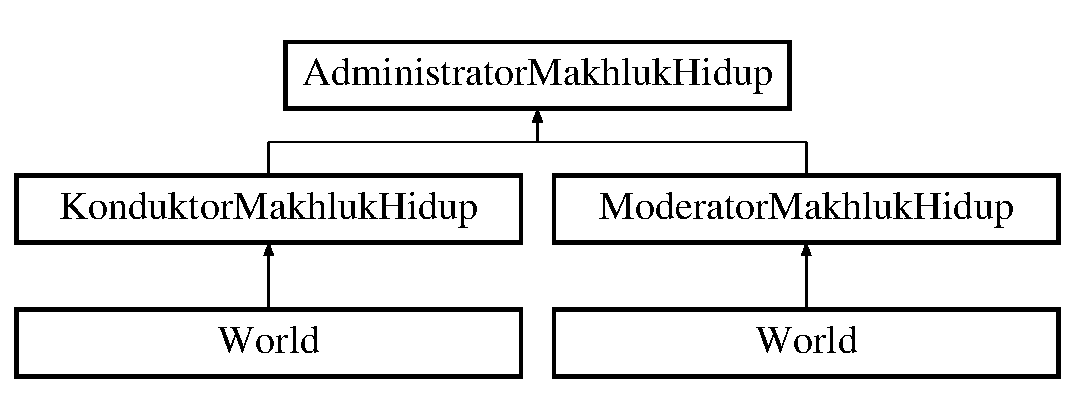
\includegraphics[height=2.000000cm]{class_administrator_makhluk_hidup}
\end{center}
\end{figure}
\subsection*{Public Member Functions}
\begin{DoxyCompactItemize}
\item 
void \hyperlink{class_administrator_makhluk_hidup_a7ce0c30393bf700eeed47fbf9c58ac04}{fill\+Daftar} (\hyperlink{class_makhluk_hidup}{Makhluk\+Hidup} $\ast$)
\item 
void \hyperlink{class_administrator_makhluk_hidup_a0766cdee6be5104128c72a6ddbc6de19}{pluck} (\hyperlink{class_makhluk_hidup}{Makhluk\+Hidup} $\ast$)
\item 
void \hyperlink{class_administrator_makhluk_hidup_a5faae20a3dfedeab6432ab0a251a7533}{pluck} (int)
\item 
void \hyperlink{class_administrator_makhluk_hidup_a9c62c4de8062108c6e7f08fc685c1e12}{sinyal} ()
\item 
int \hyperlink{class_administrator_makhluk_hidup_aa3da88881045da27c9fcb469215bce70}{get\+\_\+size} ()
\item 
int {\bfseries get\+\_\+count} ()\hypertarget{class_administrator_makhluk_hidup_a69edc3e32e43b014497a543a1e8bc1b9}{}\label{class_administrator_makhluk_hidup_a69edc3e32e43b014497a543a1e8bc1b9}

\item 
vector$<$ \hyperlink{class_makhluk_hidup}{Makhluk\+Hidup} $\ast$ $>$ {\bfseries get\+\_\+daftar} ()\hypertarget{class_administrator_makhluk_hidup_ab1a5bd8794328bad534ad07d36a8c2bb}{}\label{class_administrator_makhluk_hidup_ab1a5bd8794328bad534ad07d36a8c2bb}

\item 
\hyperlink{class_makhluk_hidup}{Makhluk\+Hidup} $\ast$ {\bfseries get\+\_\+daftar} (int i)\hypertarget{class_administrator_makhluk_hidup_aa5b4c827a367d5f533c77cd410f5575a}{}\label{class_administrator_makhluk_hidup_aa5b4c827a367d5f533c77cd410f5575a}

\item 
void {\bfseries set\+\_\+size} (int)\hypertarget{class_administrator_makhluk_hidup_a5181a812a939b545d9e183a20d1bea2f}{}\label{class_administrator_makhluk_hidup_a5181a812a939b545d9e183a20d1bea2f}

\item 
void {\bfseries set\+\_\+count} (int)\hypertarget{class_administrator_makhluk_hidup_ae196f8f31ce2dbe2be9074547e3164a0}{}\label{class_administrator_makhluk_hidup_ae196f8f31ce2dbe2be9074547e3164a0}

\end{DoxyCompactItemize}


\subsection{Detailed Description}
Class for monitoring interaction between object within the world 

\subsection{Member Function Documentation}
\index{Administrator\+Makhluk\+Hidup@{Administrator\+Makhluk\+Hidup}!fill\+Daftar@{fill\+Daftar}}
\index{fill\+Daftar@{fill\+Daftar}!Administrator\+Makhluk\+Hidup@{Administrator\+Makhluk\+Hidup}}
\subsubsection[{\texorpdfstring{fill\+Daftar(\+Makhluk\+Hidup $\ast$)}{fillDaftar(MakhlukHidup *)}}]{\setlength{\rightskip}{0pt plus 5cm}void Administrator\+Makhluk\+Hidup\+::fill\+Daftar (
\begin{DoxyParamCaption}
\item[{{\bf Makhluk\+Hidup} $\ast$}]{n}
\end{DoxyParamCaption}
)}\hypertarget{class_administrator_makhluk_hidup_a7ce0c30393bf700eeed47fbf9c58ac04}{}\label{class_administrator_makhluk_hidup_a7ce0c30393bf700eeed47fbf9c58ac04}
put in a \hyperlink{class_makhluk_hidup}{Makhluk\+Hidup} in the monitored list \index{Administrator\+Makhluk\+Hidup@{Administrator\+Makhluk\+Hidup}!get\+\_\+size@{get\+\_\+size}}
\index{get\+\_\+size@{get\+\_\+size}!Administrator\+Makhluk\+Hidup@{Administrator\+Makhluk\+Hidup}}
\subsubsection[{\texorpdfstring{get\+\_\+size()}{get_size()}}]{\setlength{\rightskip}{0pt plus 5cm}int Administrator\+Makhluk\+Hidup\+::get\+\_\+size (
\begin{DoxyParamCaption}
{}
\end{DoxyParamCaption}
)}\hypertarget{class_administrator_makhluk_hidup_aa3da88881045da27c9fcb469215bce70}{}\label{class_administrator_makhluk_hidup_aa3da88881045da27c9fcb469215bce70}
create a thread to monitor a \hyperlink{class_makhluk_hidup}{Makhluk\+Hidup} to rest of it\textquotesingle{}s peers \index{Administrator\+Makhluk\+Hidup@{Administrator\+Makhluk\+Hidup}!pluck@{pluck}}
\index{pluck@{pluck}!Administrator\+Makhluk\+Hidup@{Administrator\+Makhluk\+Hidup}}
\subsubsection[{\texorpdfstring{pluck(\+Makhluk\+Hidup $\ast$)}{pluck(MakhlukHidup *)}}]{\setlength{\rightskip}{0pt plus 5cm}void Administrator\+Makhluk\+Hidup\+::pluck (
\begin{DoxyParamCaption}
\item[{{\bf Makhluk\+Hidup} $\ast$}]{n}
\end{DoxyParamCaption}
)}\hypertarget{class_administrator_makhluk_hidup_a0766cdee6be5104128c72a6ddbc6de19}{}\label{class_administrator_makhluk_hidup_a0766cdee6be5104128c72a6ddbc6de19}
put out a \hyperlink{class_makhluk_hidup}{Makhluk\+Hidup} in the monitored list with certain pointer \index{Administrator\+Makhluk\+Hidup@{Administrator\+Makhluk\+Hidup}!pluck@{pluck}}
\index{pluck@{pluck}!Administrator\+Makhluk\+Hidup@{Administrator\+Makhluk\+Hidup}}
\subsubsection[{\texorpdfstring{pluck(int)}{pluck(int)}}]{\setlength{\rightskip}{0pt plus 5cm}void Administrator\+Makhluk\+Hidup\+::pluck (
\begin{DoxyParamCaption}
\item[{int}]{i}
\end{DoxyParamCaption}
)}\hypertarget{class_administrator_makhluk_hidup_a5faae20a3dfedeab6432ab0a251a7533}{}\label{class_administrator_makhluk_hidup_a5faae20a3dfedeab6432ab0a251a7533}
put out a \hyperlink{class_makhluk_hidup}{Makhluk\+Hidup} in the monitored list with certain index \index{Administrator\+Makhluk\+Hidup@{Administrator\+Makhluk\+Hidup}!sinyal@{sinyal}}
\index{sinyal@{sinyal}!Administrator\+Makhluk\+Hidup@{Administrator\+Makhluk\+Hidup}}
\subsubsection[{\texorpdfstring{sinyal()}{sinyal()}}]{\setlength{\rightskip}{0pt plus 5cm}void Administrator\+Makhluk\+Hidup\+::sinyal (
\begin{DoxyParamCaption}
{}
\end{DoxyParamCaption}
)}\hypertarget{class_administrator_makhluk_hidup_a9c62c4de8062108c6e7f08fc685c1e12}{}\label{class_administrator_makhluk_hidup_a9c62c4de8062108c6e7f08fc685c1e12}
create a thread to monitor each pair of \hyperlink{class_makhluk_hidup}{Makhluk\+Hidup} 

The documentation for this class was generated from the following files\+:\begin{DoxyCompactItemize}
\item 
administrator\+Makhluk\+Hidup.\+h\item 
administrator\+Makhluk\+Hidup.\+cpp\end{DoxyCompactItemize}

\hypertarget{class_burung___unta}{}\section{Burung\+\_\+\+Unta Class Reference}
\label{class_burung___unta}\index{Burung\+\_\+\+Unta@{Burung\+\_\+\+Unta}}
Inheritance diagram for Burung\+\_\+\+Unta\+:\begin{figure}[H]
\begin{center}
\leavevmode
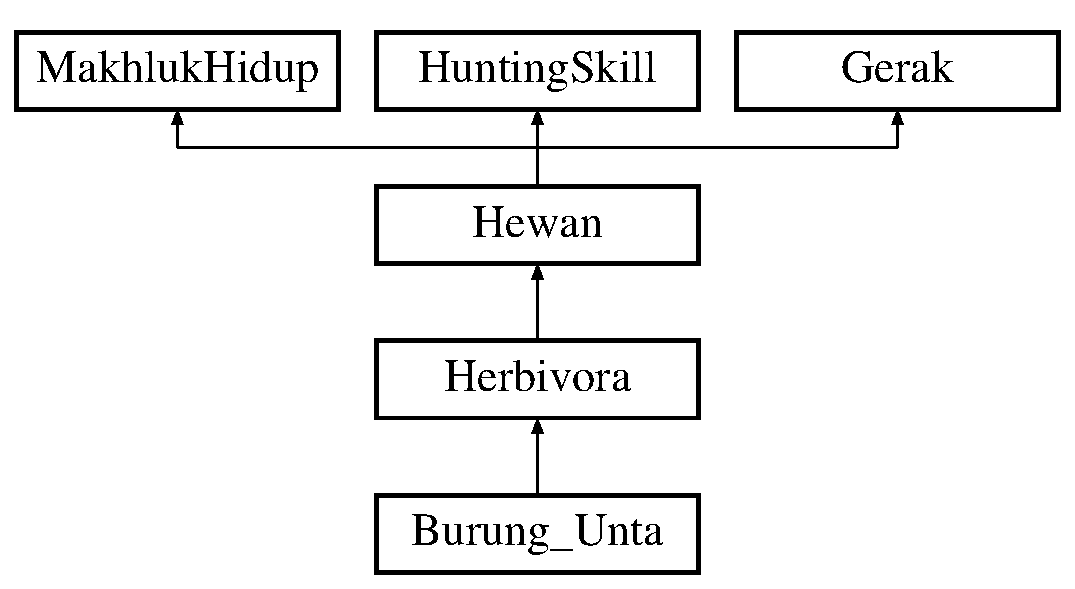
\includegraphics[height=4.000000cm]{class_burung___unta}
\end{center}
\end{figure}
\subsection*{Public Member Functions}
\begin{DoxyCompactItemize}
\item 
{\bfseries Burung\+\_\+\+Unta} (const \hyperlink{class_burung___unta}{Burung\+\_\+\+Unta} \&)\hypertarget{class_burung___unta_ab23cfda1f70b48598364c8e8baaf3732}{}\label{class_burung___unta_ab23cfda1f70b48598364c8e8baaf3732}

\item 
\hyperlink{class_burung___unta}{Burung\+\_\+\+Unta} \& {\bfseries operator=} (const \hyperlink{class_burung___unta}{Burung\+\_\+\+Unta} \&)\hypertarget{class_burung___unta_a93363d3fba519935e0dfbc537b8d8933}{}\label{class_burung___unta_a93363d3fba519935e0dfbc537b8d8933}

\item 
ifstream {\bfseries operator$>$$>$} (istream \&)\hypertarget{class_burung___unta_ae9e32d70bb8768d7d63d2b66ee4ac529}{}\label{class_burung___unta_ae9e32d70bb8768d7d63d2b66ee4ac529}

\item 
ofstream {\bfseries operator$<$$<$} (ostream \&)\hypertarget{class_burung___unta_a86ceb27cf37e0b67127ff5b0d1814a57}{}\label{class_burung___unta_a86ceb27cf37e0b67127ff5b0d1814a57}

\item 
void {\bfseries menua} ()\hypertarget{class_burung___unta_ab2937aeb5430136ba3a1407b9da21d9b}{}\label{class_burung___unta_ab2937aeb5430136ba3a1407b9da21d9b}

\item 
void {\bfseries gerak} ()\hypertarget{class_burung___unta_ae8a1e6bfdf85cf17fe75975a0454667b}{}\label{class_burung___unta_ae8a1e6bfdf85cf17fe75975a0454667b}

\item 
bool {\bfseries mati} ()\hypertarget{class_burung___unta_a2b67b21633ecc8eb281a365c187c4e0c}{}\label{class_burung___unta_a2b67b21633ecc8eb281a365c187c4e0c}

\item 
void {\bfseries display} ()\hypertarget{class_burung___unta_aba92aed2ccbd8090dddf8a8e8639ab4f}{}\label{class_burung___unta_aba92aed2ccbd8090dddf8a8e8639ab4f}

\item 
bool {\bfseries Lapar} ()\hypertarget{class_burung___unta_a054f1bc836a9c92f7dd84a6fc1e8de99}{}\label{class_burung___unta_a054f1bc836a9c92f7dd84a6fc1e8de99}

\item 
bool {\bfseries memburu} ()\hypertarget{class_burung___unta_a47d84abe318df6ee48d406acbb418f4c}{}\label{class_burung___unta_a47d84abe318df6ee48d406acbb418f4c}

\item 
bool {\bfseries berlari} ()\hypertarget{class_burung___unta_a56809a57636513f69c5c8cf2e05bb5f8}{}\label{class_burung___unta_a56809a57636513f69c5c8cf2e05bb5f8}

\end{DoxyCompactItemize}


The documentation for this class was generated from the following files\+:\begin{DoxyCompactItemize}
\item 
C\+:/\+Users/\+C\+X\+X\+X\+V/\+Documents/\+Git\+Hub/\+Makhluk/Burung\+\_\+\+Unta.\+h\item 
C\+:/\+Users/\+C\+X\+X\+X\+V/\+Documents/\+Git\+Hub/\+Makhluk/Burung\+\_\+\+Unta.\+cpp\end{DoxyCompactItemize}

\hypertarget{class_gajah}{}\section{Gajah Class Reference}
\label{class_gajah}\index{Gajah@{Gajah}}
Inheritance diagram for Gajah\+:\begin{figure}[H]
\begin{center}
\leavevmode
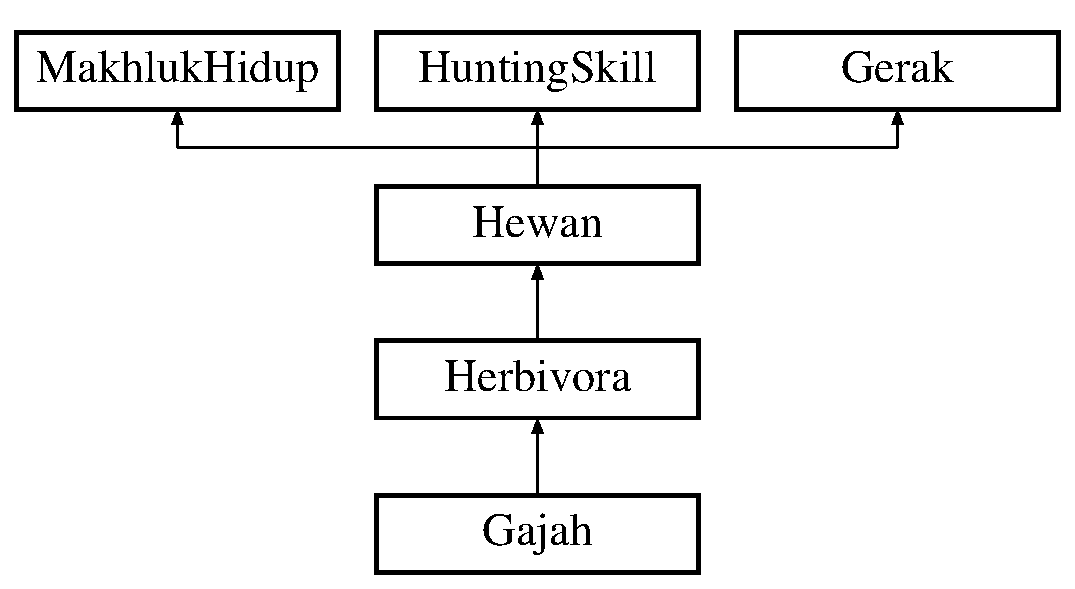
\includegraphics[height=4.000000cm]{class_gajah}
\end{center}
\end{figure}
\subsection*{Public Member Functions}
\begin{DoxyCompactItemize}
\item 
{\bfseries Gajah} (\hyperlink{class_point}{Point} P)\hypertarget{class_gajah_ad7809290b46a37d2e400d80118b985ab}{}\label{class_gajah_ad7809290b46a37d2e400d80118b985ab}

\item 
{\bfseries Gajah} (const \hyperlink{class_gajah}{Gajah} \&)\hypertarget{class_gajah_a077d7639b153d0c51bb4e458de4cbc9d}{}\label{class_gajah_a077d7639b153d0c51bb4e458de4cbc9d}

\item 
\hyperlink{class_gajah}{Gajah} \& {\bfseries operator=} (const \hyperlink{class_gajah}{Gajah} \&)\hypertarget{class_gajah_a1ec6d4ac29cf4bb30a1a4ed1faed25b4}{}\label{class_gajah_a1ec6d4ac29cf4bb30a1a4ed1faed25b4}

\item 
void \hyperlink{class_gajah_ae9f98bedbe835809f53875b234804e08}{Reaction} (\hyperlink{class_makhluk_hidup}{Makhluk\+Hidup} \&)
\end{DoxyCompactItemize}


\subsection{Member Function Documentation}
\index{Gajah@{Gajah}!Reaction@{Reaction}}
\index{Reaction@{Reaction}!Gajah@{Gajah}}
\subsubsection[{\texorpdfstring{Reaction(\+Makhluk\+Hidup \&)}{Reaction(MakhlukHidup &)}}]{\setlength{\rightskip}{0pt plus 5cm}void Gajah\+::\+Reaction (
\begin{DoxyParamCaption}
\item[{{\bf Makhluk\+Hidup} \&}]{}
\end{DoxyParamCaption}
)\hspace{0.3cm}{\ttfamily [virtual]}}\hypertarget{class_gajah_ae9f98bedbe835809f53875b234804e08}{}\label{class_gajah_ae9f98bedbe835809f53875b234804e08}
A pure virutal member 

Implements \hyperlink{class_makhluk_hidup_a7aafd6122203f48a43b384a9d8175396}{Makhluk\+Hidup}.



The documentation for this class was generated from the following files\+:\begin{DoxyCompactItemize}
\item 
Gajah.\+h\item 
Gajah.\+cpp\end{DoxyCompactItemize}

\hypertarget{class_gerak}{}\section{Gerak Class Reference}
\label{class_gerak}\index{Gerak@{Gerak}}


{\ttfamily \#include $<$Gerak.\+h$>$}

Inheritance diagram for Gerak\+:\begin{figure}[H]
\begin{center}
\leavevmode
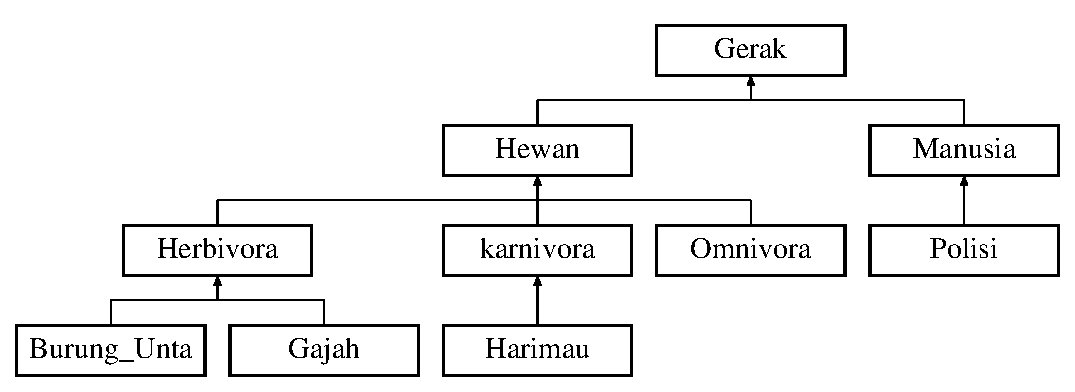
\includegraphics[height=3.255814cm]{class_gerak}
\end{center}
\end{figure}
\subsection*{Public Member Functions}
\begin{DoxyCompactItemize}
\item 
\hyperlink{class_gerak_a02d91105bf6d068a736b83cb8384771d}{Gerak} (int k=0, int a=0)
\item 
\hyperlink{class_gerak}{Gerak} \& \hyperlink{class_gerak_a305ed06e393e3e51cfca2ef6e7c76afb}{operator=} (const \hyperlink{class_gerak}{Gerak} \&)
\item 
\hyperlink{class_point}{Point} \hyperlink{class_gerak_af22d628d35499daa0531c7ec33bc203c}{gerak\+\_\+bebas} (\hyperlink{class_point}{Point} Awal)
\item 
\hyperlink{class_point}{Point} \hyperlink{class_gerak_ad5580d6323e4c6b4ef8df2b66ae0e3d4}{gerak\+\_\+memburu} (\hyperlink{class_point}{Point} Awal, \hyperlink{class_point}{Point} Target)
\item 
\hyperlink{class_point}{Point} \hyperlink{class_gerak_a35bd72ee39648608e80e3a6e64529629}{gerak\+\_\+menjauh} (\hyperlink{class_point}{Point} Awal, \hyperlink{class_point}{Point} Predator)
\item 
\hyperlink{class_point}{Point} \hyperlink{class_gerak_a523d205606d855b9776ef64f92cc756e}{gerak\+\_\+berarah} (\hyperlink{class_point}{Point} Awal)
\item 
void \hyperlink{class_gerak_aeb2593139ccb712e979d2be884f7b964}{set\+\_\+\+Kecepatan} (int \+\_\+kecepatan)
\item 
void \hyperlink{class_gerak_a79f2c0d4777b7fdf7828783b4b6ebf59}{set\+\_\+\+Arah} (int \+\_\+arah)
\item 
void \hyperlink{class_gerak_a2b06276ef18ad27ab8cbe71655e9c198}{set\+\_\+\+Arah\+\_\+\+Bebas} ()
\item 
void \hyperlink{class_gerak_a0d31d49a0104e4d823bbfc2881a0f599}{set\+\_\+\+Arah\+\_\+\+Memburu} (\hyperlink{class_point}{Point} Awal, \hyperlink{class_point}{Point} Target)
\item 
void \hyperlink{class_gerak_a8a5617adee7b2c7d67b0f4571ca4b448}{set\+\_\+\+Arah\+\_\+\+Menjauh} (\hyperlink{class_point}{Point} Awal, \hyperlink{class_point}{Point} Predator)
\item 
int \hyperlink{class_gerak_a7c19aee88213b75f332d286458069ccd}{get\+\_\+\+Kecepatan} ()
\item 
int \hyperlink{class_gerak_ae808d0044c5221cf7e265fb43288b51b}{get\+\_\+\+Arah} ()
\end{DoxyCompactItemize}


\subsection{Detailed Description}
A gerak class. A class that describe a movement. 

\subsection{Constructor \& Destructor Documentation}
\index{Gerak@{Gerak}!Gerak@{Gerak}}
\index{Gerak@{Gerak}!Gerak@{Gerak}}
\subsubsection[{\texorpdfstring{Gerak(int k=0, int a=0)}{Gerak(int k=0, int a=0)}}]{\setlength{\rightskip}{0pt plus 5cm}Gerak\+::\+Gerak (
\begin{DoxyParamCaption}
\item[{int}]{k = {\ttfamily 0}, }
\item[{int}]{a = {\ttfamily 0}}
\end{DoxyParamCaption}
)}\hypertarget{class_gerak_a02d91105bf6d068a736b83cb8384771d}{}\label{class_gerak_a02d91105bf6d068a736b83cb8384771d}
A constructor. Making a movement with default parameter value in every parameter. 
\begin{DoxyParams}{Parameters}
{\em k} & A parameter that will be assign to direction. \\
\hline
{\em a} & A parameter that will be assign to velocity. \\
\hline
\end{DoxyParams}


\subsection{Member Function Documentation}
\index{Gerak@{Gerak}!gerak\+\_\+bebas@{gerak\+\_\+bebas}}
\index{gerak\+\_\+bebas@{gerak\+\_\+bebas}!Gerak@{Gerak}}
\subsubsection[{\texorpdfstring{gerak\+\_\+bebas(\+Point Awal)}{gerak_bebas(Point Awal)}}]{\setlength{\rightskip}{0pt plus 5cm}{\bf Point} Gerak\+::gerak\+\_\+bebas (
\begin{DoxyParamCaption}
\item[{{\bf Point}}]{Awal}
\end{DoxyParamCaption}
)}\hypertarget{class_gerak_af22d628d35499daa0531c7ec33bc203c}{}\label{class_gerak_af22d628d35499daa0531c7ec33bc203c}
A movement function returns a new cordinate. This movement use random direction. It just can move in one block. 
\begin{DoxyParams}{Parameters}
{\em Awal} & Awal parameter that describe the first cordinate. \\
\hline
\end{DoxyParams}
\begin{DoxyReturn}{Returns}
a \hyperlink{class_point}{Point}, new cordinate 
\end{DoxyReturn}
\index{Gerak@{Gerak}!gerak\+\_\+berarah@{gerak\+\_\+berarah}}
\index{gerak\+\_\+berarah@{gerak\+\_\+berarah}!Gerak@{Gerak}}
\subsubsection[{\texorpdfstring{gerak\+\_\+berarah(\+Point Awal)}{gerak_berarah(Point Awal)}}]{\setlength{\rightskip}{0pt plus 5cm}{\bf Point} Gerak\+::gerak\+\_\+berarah (
\begin{DoxyParamCaption}
\item[{{\bf Point}}]{Awal}
\end{DoxyParamCaption}
)}\hypertarget{class_gerak_a523d205606d855b9776ef64f92cc756e}{}\label{class_gerak_a523d205606d855b9776ef64f92cc756e}
A movement function returns a new cordinate. This movement use direction which get from attribute. It just can move in one block 
\begin{DoxyParams}{Parameters}
{\em Awal} & Awal parameter that describe the first cordinate. \\
\hline
\end{DoxyParams}
\begin{DoxyReturn}{Returns}
a \hyperlink{class_point}{Point}, new cordinate 
\end{DoxyReturn}
\index{Gerak@{Gerak}!gerak\+\_\+memburu@{gerak\+\_\+memburu}}
\index{gerak\+\_\+memburu@{gerak\+\_\+memburu}!Gerak@{Gerak}}
\subsubsection[{\texorpdfstring{gerak\+\_\+memburu(\+Point Awal, Point Target)}{gerak_memburu(Point Awal, Point Target)}}]{\setlength{\rightskip}{0pt plus 5cm}{\bf Point} Gerak\+::gerak\+\_\+memburu (
\begin{DoxyParamCaption}
\item[{{\bf Point}}]{Awal, }
\item[{{\bf Point}}]{Target}
\end{DoxyParamCaption}
)}\hypertarget{class_gerak_ad5580d6323e4c6b4ef8df2b66ae0e3d4}{}\label{class_gerak_ad5580d6323e4c6b4ef8df2b66ae0e3d4}
A movement function returns a new cordinate. This movement use direction which close to target. It just can move in one block 
\begin{DoxyParams}{Parameters}
{\em Awal} & parameter that describe the first cordinate. \\
\hline
{\em Target} & Target parameter that describe the cordinate of target. \\
\hline
\end{DoxyParams}
\begin{DoxyReturn}{Returns}
a \hyperlink{class_point}{Point}, new cordinate 
\end{DoxyReturn}
\index{Gerak@{Gerak}!gerak\+\_\+menjauh@{gerak\+\_\+menjauh}}
\index{gerak\+\_\+menjauh@{gerak\+\_\+menjauh}!Gerak@{Gerak}}
\subsubsection[{\texorpdfstring{gerak\+\_\+menjauh(\+Point Awal, Point Predator)}{gerak_menjauh(Point Awal, Point Predator)}}]{\setlength{\rightskip}{0pt plus 5cm}{\bf Point} Gerak\+::gerak\+\_\+menjauh (
\begin{DoxyParamCaption}
\item[{{\bf Point}}]{Awal, }
\item[{{\bf Point}}]{Predator}
\end{DoxyParamCaption}
)}\hypertarget{class_gerak_a35bd72ee39648608e80e3a6e64529629}{}\label{class_gerak_a35bd72ee39648608e80e3a6e64529629}
A movement function returns a new cordinate. This movement use direction which away from target. It just can move in one block 
\begin{DoxyParams}{Parameters}
{\em Awal} & parameter that describe the first cordinate. \\
\hline
{\em Predator} & parameter that describe the cordinate of predator. \\
\hline
\end{DoxyParams}
\begin{DoxyReturn}{Returns}
a \hyperlink{class_point}{Point}, new cordinate 
\end{DoxyReturn}
\index{Gerak@{Gerak}!get\+\_\+\+Arah@{get\+\_\+\+Arah}}
\index{get\+\_\+\+Arah@{get\+\_\+\+Arah}!Gerak@{Gerak}}
\subsubsection[{\texorpdfstring{get\+\_\+\+Arah()}{get_Arah()}}]{\setlength{\rightskip}{0pt plus 5cm}int Gerak\+::get\+\_\+\+Arah (
\begin{DoxyParamCaption}
{}
\end{DoxyParamCaption}
)}\hypertarget{class_gerak_ae808d0044c5221cf7e265fb43288b51b}{}\label{class_gerak_ae808d0044c5221cf7e265fb43288b51b}
A getter for Kecepatan \begin{DoxyReturn}{Returns}
an integer, direction 
\end{DoxyReturn}
\index{Gerak@{Gerak}!get\+\_\+\+Kecepatan@{get\+\_\+\+Kecepatan}}
\index{get\+\_\+\+Kecepatan@{get\+\_\+\+Kecepatan}!Gerak@{Gerak}}
\subsubsection[{\texorpdfstring{get\+\_\+\+Kecepatan()}{get_Kecepatan()}}]{\setlength{\rightskip}{0pt plus 5cm}int Gerak\+::get\+\_\+\+Kecepatan (
\begin{DoxyParamCaption}
{}
\end{DoxyParamCaption}
)}\hypertarget{class_gerak_a7c19aee88213b75f332d286458069ccd}{}\label{class_gerak_a7c19aee88213b75f332d286458069ccd}
A getter for Kecepatan \begin{DoxyReturn}{Returns}
an integer, velocity 
\end{DoxyReturn}
\index{Gerak@{Gerak}!operator=@{operator=}}
\index{operator=@{operator=}!Gerak@{Gerak}}
\subsubsection[{\texorpdfstring{operator=(const Gerak \&)}{operator=(const Gerak &)}}]{\setlength{\rightskip}{0pt plus 5cm}{\bf Gerak} \& Gerak\+::operator= (
\begin{DoxyParamCaption}
\item[{const {\bf Gerak} \&}]{G}
\end{DoxyParamCaption}
)}\hypertarget{class_gerak_a305ed06e393e3e51cfca2ef6e7c76afb}{}\label{class_gerak_a305ed06e393e3e51cfca2ef6e7c76afb}
An Operator = \index{Gerak@{Gerak}!set\+\_\+\+Arah@{set\+\_\+\+Arah}}
\index{set\+\_\+\+Arah@{set\+\_\+\+Arah}!Gerak@{Gerak}}
\subsubsection[{\texorpdfstring{set\+\_\+\+Arah(int \+\_\+arah)}{set_Arah(int _arah)}}]{\setlength{\rightskip}{0pt plus 5cm}void Gerak\+::set\+\_\+\+Arah (
\begin{DoxyParamCaption}
\item[{int}]{\+\_\+arah}
\end{DoxyParamCaption}
)}\hypertarget{class_gerak_a79f2c0d4777b7fdf7828783b4b6ebf59}{}\label{class_gerak_a79f2c0d4777b7fdf7828783b4b6ebf59}
A setter for Arah. 
\begin{DoxyParams}{Parameters}
{\em a} & int argument that will be assigned to dircetion. It has value between 1 to 8. \\
\hline
\end{DoxyParams}
\index{Gerak@{Gerak}!set\+\_\+\+Arah\+\_\+\+Bebas@{set\+\_\+\+Arah\+\_\+\+Bebas}}
\index{set\+\_\+\+Arah\+\_\+\+Bebas@{set\+\_\+\+Arah\+\_\+\+Bebas}!Gerak@{Gerak}}
\subsubsection[{\texorpdfstring{set\+\_\+\+Arah\+\_\+\+Bebas()}{set_Arah_Bebas()}}]{\setlength{\rightskip}{0pt plus 5cm}void Gerak\+::set\+\_\+\+Arah\+\_\+\+Bebas (
\begin{DoxyParamCaption}
{}
\end{DoxyParamCaption}
)}\hypertarget{class_gerak_a2b06276ef18ad27ab8cbe71655e9c198}{}\label{class_gerak_a2b06276ef18ad27ab8cbe71655e9c198}
A setter for Arah. Set direction attribute with random integer which has value between 1 to 8. \index{Gerak@{Gerak}!set\+\_\+\+Arah\+\_\+\+Memburu@{set\+\_\+\+Arah\+\_\+\+Memburu}}
\index{set\+\_\+\+Arah\+\_\+\+Memburu@{set\+\_\+\+Arah\+\_\+\+Memburu}!Gerak@{Gerak}}
\subsubsection[{\texorpdfstring{set\+\_\+\+Arah\+\_\+\+Memburu(\+Point Awal, Point Target)}{set_Arah_Memburu(Point Awal, Point Target)}}]{\setlength{\rightskip}{0pt plus 5cm}void Gerak\+::set\+\_\+\+Arah\+\_\+\+Memburu (
\begin{DoxyParamCaption}
\item[{{\bf Point}}]{Awal, }
\item[{{\bf Point}}]{Target}
\end{DoxyParamCaption}
)}\hypertarget{class_gerak_a0d31d49a0104e4d823bbfc2881a0f599}{}\label{class_gerak_a0d31d49a0104e4d823bbfc2881a0f599}
A setter for Arah. Set direction attribute with integer which references direction from origin to destination 
\begin{DoxyParams}{Parameters}
{\em Awal} & A point argument describe the origin \\
\hline
{\em Target} & A point argument describe the destination. \\
\hline
\end{DoxyParams}
\index{Gerak@{Gerak}!set\+\_\+\+Arah\+\_\+\+Menjauh@{set\+\_\+\+Arah\+\_\+\+Menjauh}}
\index{set\+\_\+\+Arah\+\_\+\+Menjauh@{set\+\_\+\+Arah\+\_\+\+Menjauh}!Gerak@{Gerak}}
\subsubsection[{\texorpdfstring{set\+\_\+\+Arah\+\_\+\+Menjauh(\+Point Awal, Point Predator)}{set_Arah_Menjauh(Point Awal, Point Predator)}}]{\setlength{\rightskip}{0pt plus 5cm}void Gerak\+::set\+\_\+\+Arah\+\_\+\+Menjauh (
\begin{DoxyParamCaption}
\item[{{\bf Point}}]{Awal, }
\item[{{\bf Point}}]{Predator}
\end{DoxyParamCaption}
)}\hypertarget{class_gerak_a8a5617adee7b2c7d67b0f4571ca4b448}{}\label{class_gerak_a8a5617adee7b2c7d67b0f4571ca4b448}
A setter for Arah. Set direction attribute with integer which references direction which away from predator 
\begin{DoxyParams}{Parameters}
{\em Awal} & A point argument describe the origin \\
\hline
{\em Predator} & A point argument describe the predator. \\
\hline
\end{DoxyParams}
\index{Gerak@{Gerak}!set\+\_\+\+Kecepatan@{set\+\_\+\+Kecepatan}}
\index{set\+\_\+\+Kecepatan@{set\+\_\+\+Kecepatan}!Gerak@{Gerak}}
\subsubsection[{\texorpdfstring{set\+\_\+\+Kecepatan(int \+\_\+kecepatan)}{set_Kecepatan(int _kecepatan)}}]{\setlength{\rightskip}{0pt plus 5cm}void Gerak\+::set\+\_\+\+Kecepatan (
\begin{DoxyParamCaption}
\item[{int}]{\+\_\+kecepatan}
\end{DoxyParamCaption}
)}\hypertarget{class_gerak_aeb2593139ccb712e979d2be884f7b964}{}\label{class_gerak_aeb2593139ccb712e979d2be884f7b964}
A setter for Kecepatan. 
\begin{DoxyParams}{Parameters}
{\em a} & int argument that will be assigned to velocity. \\
\hline
\end{DoxyParams}


The documentation for this class was generated from the following files\+:\begin{DoxyCompactItemize}
\item 
Gerak.\+h\item 
Gerak.\+cpp\end{DoxyCompactItemize}

\hypertarget{class_harimau}{}\section{Harimau Class Reference}
\label{class_harimau}\index{Harimau@{Harimau}}


{\ttfamily \#include $<$harimau.\+h$>$}

Inheritance diagram for Harimau\+:\begin{figure}[H]
\begin{center}
\leavevmode
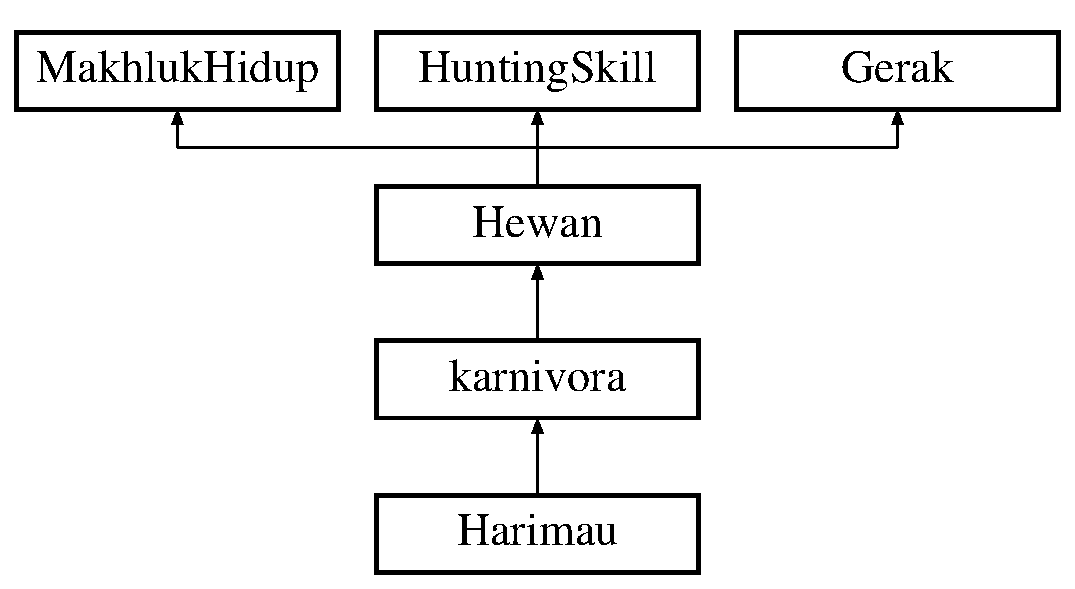
\includegraphics[height=4.000000cm]{class_harimau}
\end{center}
\end{figure}
\subsection*{Public Member Functions}
\begin{DoxyCompactItemize}
\item 
\hyperlink{class_harimau_a42b5e71cced7feb81542646f98811b98}{Harimau} (\hyperlink{class_point}{Point} P)
\item 
\hyperlink{class_harimau_a0c9d5174a7f6b6bfaa3e7b5c009b32dc}{Harimau} (const \hyperlink{class_harimau}{Harimau} \&)
\item 
\hyperlink{class_harimau_a2cd850b67b1b4849cd8bfc92b122aab3}{$\sim$\+Harimau} ()
\item 
\hyperlink{class_harimau}{Harimau} \& \hyperlink{class_harimau_ab9fc093228616066efb58f2f1f9b601c}{operator=} (const \hyperlink{class_harimau}{Harimau} \&)
\end{DoxyCompactItemize}


\subsection{Detailed Description}
Class for constructing a carnivore called \hyperlink{class_harimau}{Harimau} 

\subsection{Constructor \& Destructor Documentation}
\index{Harimau@{Harimau}!Harimau@{Harimau}}
\index{Harimau@{Harimau}!Harimau@{Harimau}}
\subsubsection[{\texorpdfstring{Harimau(\+Point P)}{Harimau(Point P)}}]{\setlength{\rightskip}{0pt plus 5cm}Harimau\+::\+Harimau (
\begin{DoxyParamCaption}
\item[{{\bf Point}}]{P}
\end{DoxyParamCaption}
)}\hypertarget{class_harimau_a42b5e71cced7feb81542646f98811b98}{}\label{class_harimau_a42b5e71cced7feb81542646f98811b98}
ctor that take one argument to set the position of the \hyperlink{class_harimau}{Harimau} 
\begin{DoxyParams}{Parameters}
{\em A} & \hyperlink{class_point}{Point} \\
\hline
\end{DoxyParams}
\index{Harimau@{Harimau}!Harimau@{Harimau}}
\index{Harimau@{Harimau}!Harimau@{Harimau}}
\subsubsection[{\texorpdfstring{Harimau(const Harimau \&)}{Harimau(const Harimau &)}}]{\setlength{\rightskip}{0pt plus 5cm}Harimau\+::\+Harimau (
\begin{DoxyParamCaption}
\item[{const {\bf Harimau} \&}]{H}
\end{DoxyParamCaption}
)}\hypertarget{class_harimau_a0c9d5174a7f6b6bfaa3e7b5c009b32dc}{}\label{class_harimau_a0c9d5174a7f6b6bfaa3e7b5c009b32dc}
a copy construktor \index{Harimau@{Harimau}!````~Harimau@{$\sim$\+Harimau}}
\index{````~Harimau@{$\sim$\+Harimau}!Harimau@{Harimau}}
\subsubsection[{\texorpdfstring{$\sim$\+Harimau()}{~Harimau()}}]{\setlength{\rightskip}{0pt plus 5cm}Harimau\+::$\sim$\+Harimau (
\begin{DoxyParamCaption}
{}
\end{DoxyParamCaption}
)}\hypertarget{class_harimau_a2cd850b67b1b4849cd8bfc92b122aab3}{}\label{class_harimau_a2cd850b67b1b4849cd8bfc92b122aab3}
a destructor 

\subsection{Member Function Documentation}
\index{Harimau@{Harimau}!operator=@{operator=}}
\index{operator=@{operator=}!Harimau@{Harimau}}
\subsubsection[{\texorpdfstring{operator=(const Harimau \&)}{operator=(const Harimau &)}}]{\setlength{\rightskip}{0pt plus 5cm}{\bf Harimau} \& Harimau\+::operator= (
\begin{DoxyParamCaption}
\item[{const {\bf Harimau} \&}]{H}
\end{DoxyParamCaption}
)}\hypertarget{class_harimau_ab9fc093228616066efb58f2f1f9b601c}{}\label{class_harimau_ab9fc093228616066efb58f2f1f9b601c}
an operator= 

The documentation for this class was generated from the following files\+:\begin{DoxyCompactItemize}
\item 
harimau.\+h\item 
Harimau.\+cpp\end{DoxyCompactItemize}

\hypertarget{class_herbivora}{}\section{Herbivora Class Reference}
\label{class_herbivora}\index{Herbivora@{Herbivora}}


{\ttfamily \#include $<$Herbivora.\+h$>$}

Inheritance diagram for Herbivora\+:\begin{figure}[H]
\begin{center}
\leavevmode
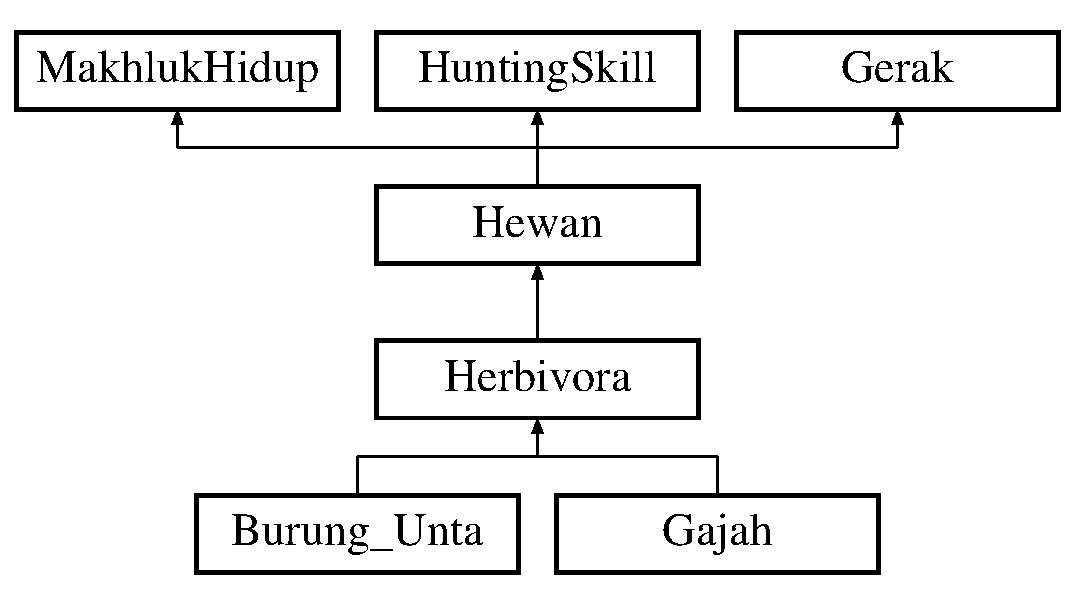
\includegraphics[height=4.000000cm]{class_herbivora}
\end{center}
\end{figure}
\subsection*{Public Member Functions}
\begin{DoxyCompactItemize}
\item 
\hyperlink{class_herbivora_ae8610577ee87a166177be431b989b2c0}{Herbivora} ()
\item 
\hyperlink{class_herbivora_a226a2efa9d41653fab8efa87608b583d}{Herbivora} (int \+\_\+umur, char \+\_\+\+D\+NA, int \+\_\+ulangtahun, \hyperlink{class_point}{Point} P, int kenyang, int maks, char $\ast$tar, bool \+\_\+memburu, int k, int a, bool lambat, int delta)
\item 
\hyperlink{class_herbivora_a754ef435d7a6a6bffe727e809e5f211b}{Herbivora} (const \hyperlink{class_herbivora}{Herbivora} \&)
\item 
\hyperlink{class_herbivora}{Herbivora} \& \hyperlink{class_herbivora_a045acf6e3df5988ca9e93384e5450876}{operator=} (const \hyperlink{class_herbivora}{Herbivora} \&)
\item 
virtual \hyperlink{class_herbivora_aa0dcb5298f0e99b7bcb1a335bdffa393}{$\sim$\+Herbivora} ()
\item 
void \hyperlink{class_herbivora_a1b460ec339813b44bd368412fd3b2c76}{set\+\_\+percepat} (bool cepat)
\item 
void \hyperlink{class_herbivora_a8cf1ea08fd33527b16e2092935080a3d}{set\+\_\+delta\+Kecepatan} (int kec)
\item 
bool \hyperlink{class_herbivora_acf023d22ffa5accee04a503ded9952a6}{get\+\_\+percepat} ()
\item 
int \hyperlink{class_herbivora_a60f1095412a18804afd582dbba89415b}{get\+\_\+delta\+Kecepatan} ()
\item 
void \hyperlink{class_herbivora_a8e90ec668b96032f698bf99569481f62}{proses\+Mempercepat} ()
\item 
virtual void \hyperlink{class_herbivora_a649b50a3d1e6f8d290baf1977a6ce88a}{Reaction} (\hyperlink{class_makhluk_hidup}{Makhluk\+Hidup} \&)
\end{DoxyCompactItemize}


\subsection{Detailed Description}
Class that describes Herbivore animals. 

\subsection{Constructor \& Destructor Documentation}
\index{Herbivora@{Herbivora}!Herbivora@{Herbivora}}
\index{Herbivora@{Herbivora}!Herbivora@{Herbivora}}
\subsubsection[{\texorpdfstring{Herbivora()}{Herbivora()}}]{\setlength{\rightskip}{0pt plus 5cm}Herbivora\+::\+Herbivora (
\begin{DoxyParamCaption}
{}
\end{DoxyParamCaption}
)}\hypertarget{class_herbivora_ae8610577ee87a166177be431b989b2c0}{}\label{class_herbivora_ae8610577ee87a166177be431b989b2c0}
constructor with no parameter \index{Herbivora@{Herbivora}!Herbivora@{Herbivora}}
\index{Herbivora@{Herbivora}!Herbivora@{Herbivora}}
\subsubsection[{\texorpdfstring{Herbivora(int \+\_\+umur, char \+\_\+\+D\+N\+A, int \+\_\+ulangtahun, Point P, int kenyang, int maks, char $\ast$tar, bool \+\_\+memburu, int k, int a, bool lambat, int delta)}{Herbivora(int _umur, char _DNA, int _ulangtahun, Point P, int kenyang, int maks, char *tar, bool _memburu, int k, int a, bool lambat, int delta)}}]{\setlength{\rightskip}{0pt plus 5cm}Herbivora\+::\+Herbivora (
\begin{DoxyParamCaption}
\item[{int}]{\+\_\+umur, }
\item[{char}]{\+\_\+\+D\+NA, }
\item[{int}]{\+\_\+ulangtahun, }
\item[{{\bf Point}}]{P, }
\item[{int}]{kenyang, }
\item[{int}]{maks, }
\item[{char $\ast$}]{tar, }
\item[{bool}]{\+\_\+memburu, }
\item[{int}]{k, }
\item[{int}]{a, }
\item[{bool}]{lambat, }
\item[{int}]{delta}
\end{DoxyParamCaption}
)}\hypertarget{class_herbivora_a226a2efa9d41653fab8efa87608b583d}{}\label{class_herbivora_a226a2efa9d41653fab8efa87608b583d}
A constructor that take 12 parameter 
\begin{DoxyParams}{Parameters}
{\em an} & integer for the age limit of the herbivore \\
\hline
{\em a} & character of the herbivore\textquotesingle{}s D\+NA \\
\hline
{\em an} & integer \char`\"{}birthday\char`\"{} that saves the birthday time for herbivore \\
\hline
{\em a} & \hyperlink{class_point}{Point} that tells the position of the Hernivore \\
\hline
{\em an} & integer that set \char`\"{}tingkat\+\_\+kekenyangan\char`\"{} \\
\hline
{\em an} & integer that set \char`\"{}maks\+\_\+tingkat\+\_\+kekenyangan\char`\"{} \\
\hline
{\em a} & character pointer that contain prey of the herbivore \\
\hline
{\em a} & boolean, the hunting state of the herbivore \\
\hline
{\em an} & integer k, contain the herbivore velocity \\
\hline
{\em an} & integer a, contain the herbivore first move default direction \\
\hline
{\em a} & boolean, the state that the tell whether the herbivore is slowed or not \\
\hline
{\em an} & integer that contain the acceleration of the herbivore \\
\hline
\end{DoxyParams}
\index{Herbivora@{Herbivora}!Herbivora@{Herbivora}}
\index{Herbivora@{Herbivora}!Herbivora@{Herbivora}}
\subsubsection[{\texorpdfstring{Herbivora(const Herbivora \&)}{Herbivora(const Herbivora &)}}]{\setlength{\rightskip}{0pt plus 5cm}Herbivora\+::\+Herbivora (
\begin{DoxyParamCaption}
\item[{const {\bf Herbivora} \&}]{H}
\end{DoxyParamCaption}
)}\hypertarget{class_herbivora_a754ef435d7a6a6bffe727e809e5f211b}{}\label{class_herbivora_a754ef435d7a6a6bffe727e809e5f211b}
A copy constructor \index{Herbivora@{Herbivora}!````~Herbivora@{$\sim$\+Herbivora}}
\index{````~Herbivora@{$\sim$\+Herbivora}!Herbivora@{Herbivora}}
\subsubsection[{\texorpdfstring{$\sim$\+Herbivora()}{~Herbivora()}}]{\setlength{\rightskip}{0pt plus 5cm}Herbivora\+::$\sim$\+Herbivora (
\begin{DoxyParamCaption}
{}
\end{DoxyParamCaption}
)\hspace{0.3cm}{\ttfamily [virtual]}}\hypertarget{class_herbivora_aa0dcb5298f0e99b7bcb1a335bdffa393}{}\label{class_herbivora_aa0dcb5298f0e99b7bcb1a335bdffa393}
a virtual destructor 

\subsection{Member Function Documentation}
\index{Herbivora@{Herbivora}!get\+\_\+delta\+Kecepatan@{get\+\_\+delta\+Kecepatan}}
\index{get\+\_\+delta\+Kecepatan@{get\+\_\+delta\+Kecepatan}!Herbivora@{Herbivora}}
\subsubsection[{\texorpdfstring{get\+\_\+delta\+Kecepatan()}{get_deltaKecepatan()}}]{\setlength{\rightskip}{0pt plus 5cm}int Herbivora\+::get\+\_\+delta\+Kecepatan (
\begin{DoxyParamCaption}
{}
\end{DoxyParamCaption}
)}\hypertarget{class_herbivora_a60f1095412a18804afd582dbba89415b}{}\label{class_herbivora_a60f1095412a18804afd582dbba89415b}
get the acceleration \begin{DoxyReturn}{Returns}
an integer 
\end{DoxyReturn}
\index{Herbivora@{Herbivora}!get\+\_\+percepat@{get\+\_\+percepat}}
\index{get\+\_\+percepat@{get\+\_\+percepat}!Herbivora@{Herbivora}}
\subsubsection[{\texorpdfstring{get\+\_\+percepat()}{get_percepat()}}]{\setlength{\rightskip}{0pt plus 5cm}bool Herbivora\+::get\+\_\+percepat (
\begin{DoxyParamCaption}
{}
\end{DoxyParamCaption}
)}\hypertarget{class_herbivora_acf023d22ffa5accee04a503ded9952a6}{}\label{class_herbivora_acf023d22ffa5accee04a503ded9952a6}
get the state of the Herbivore 
\begin{DoxyParams}{Parameters}
{\em a} & boolean, true if the Herbivore is accelerated \\
\hline
\end{DoxyParams}
\index{Herbivora@{Herbivora}!operator=@{operator=}}
\index{operator=@{operator=}!Herbivora@{Herbivora}}
\subsubsection[{\texorpdfstring{operator=(const Herbivora \&)}{operator=(const Herbivora &)}}]{\setlength{\rightskip}{0pt plus 5cm}{\bf Herbivora} \& Herbivora\+::operator= (
\begin{DoxyParamCaption}
\item[{const {\bf Herbivora} \&}]{H}
\end{DoxyParamCaption}
)}\hypertarget{class_herbivora_a045acf6e3df5988ca9e93384e5450876}{}\label{class_herbivora_a045acf6e3df5988ca9e93384e5450876}
an operator= \index{Herbivora@{Herbivora}!proses\+Mempercepat@{proses\+Mempercepat}}
\index{proses\+Mempercepat@{proses\+Mempercepat}!Herbivora@{Herbivora}}
\subsubsection[{\texorpdfstring{proses\+Mempercepat()}{prosesMempercepat()}}]{\setlength{\rightskip}{0pt plus 5cm}void Herbivora\+::proses\+Mempercepat (
\begin{DoxyParamCaption}
{}
\end{DoxyParamCaption}
)}\hypertarget{class_herbivora_a8e90ec668b96032f698bf99569481f62}{}\label{class_herbivora_a8e90ec668b96032f698bf99569481f62}
a procedure to simulate how the herbivore move faster \index{Herbivora@{Herbivora}!Reaction@{Reaction}}
\index{Reaction@{Reaction}!Herbivora@{Herbivora}}
\subsubsection[{\texorpdfstring{Reaction(\+Makhluk\+Hidup \&)}{Reaction(MakhlukHidup &)}}]{\setlength{\rightskip}{0pt plus 5cm}void Herbivora\+::\+Reaction (
\begin{DoxyParamCaption}
\item[{{\bf Makhluk\+Hidup} \&}]{M}
\end{DoxyParamCaption}
)\hspace{0.3cm}{\ttfamily [virtual]}}\hypertarget{class_herbivora_a649b50a3d1e6f8d290baf1977a6ce88a}{}\label{class_herbivora_a649b50a3d1e6f8d290baf1977a6ce88a}
a procedure that makes herbivore react to its environment Herbivore can eat, or going faster to flee away from its predator 
\begin{DoxyParams}{Parameters}
{\em a} & \hyperlink{class_makhluk_hidup}{Makhluk\+Hidup}, another \hyperlink{class_makhluk_hidup}{Makhluk\+Hidup} near the Herbivore \\
\hline
\end{DoxyParams}


Implements \hyperlink{class_makhluk_hidup_a7aafd6122203f48a43b384a9d8175396}{Makhluk\+Hidup}.



Reimplemented in \hyperlink{class_burung_unta_afbf850167abdb1d2912284cccb497c13}{Burung\+Unta}, and \hyperlink{class_gajah_ae9f98bedbe835809f53875b234804e08}{Gajah}.

\index{Herbivora@{Herbivora}!set\+\_\+delta\+Kecepatan@{set\+\_\+delta\+Kecepatan}}
\index{set\+\_\+delta\+Kecepatan@{set\+\_\+delta\+Kecepatan}!Herbivora@{Herbivora}}
\subsubsection[{\texorpdfstring{set\+\_\+delta\+Kecepatan(int kec)}{set_deltaKecepatan(int kec)}}]{\setlength{\rightskip}{0pt plus 5cm}void Herbivora\+::set\+\_\+delta\+Kecepatan (
\begin{DoxyParamCaption}
\item[{int}]{kec}
\end{DoxyParamCaption}
)}\hypertarget{class_herbivora_a8cf1ea08fd33527b16e2092935080a3d}{}\label{class_herbivora_a8cf1ea08fd33527b16e2092935080a3d}
set the acceleration \index{Herbivora@{Herbivora}!set\+\_\+percepat@{set\+\_\+percepat}}
\index{set\+\_\+percepat@{set\+\_\+percepat}!Herbivora@{Herbivora}}
\subsubsection[{\texorpdfstring{set\+\_\+percepat(bool cepat)}{set_percepat(bool cepat)}}]{\setlength{\rightskip}{0pt plus 5cm}void Herbivora\+::set\+\_\+percepat (
\begin{DoxyParamCaption}
\item[{bool}]{cepat}
\end{DoxyParamCaption}
)}\hypertarget{class_herbivora_a1b460ec339813b44bd368412fd3b2c76}{}\label{class_herbivora_a1b460ec339813b44bd368412fd3b2c76}
set the state of the Herbivore to Accelerated or not 

The documentation for this class was generated from the following files\+:\begin{DoxyCompactItemize}
\item 
Herbivora.\+h\item 
Herbivora.\+cpp\end{DoxyCompactItemize}

\hypertarget{class_hewan}{}\section{Hewan Class Reference}
\label{class_hewan}\index{Hewan@{Hewan}}


{\ttfamily \#include $<$Hewan.\+h$>$}

Inheritance diagram for Hewan\+:\begin{figure}[H]
\begin{center}
\leavevmode
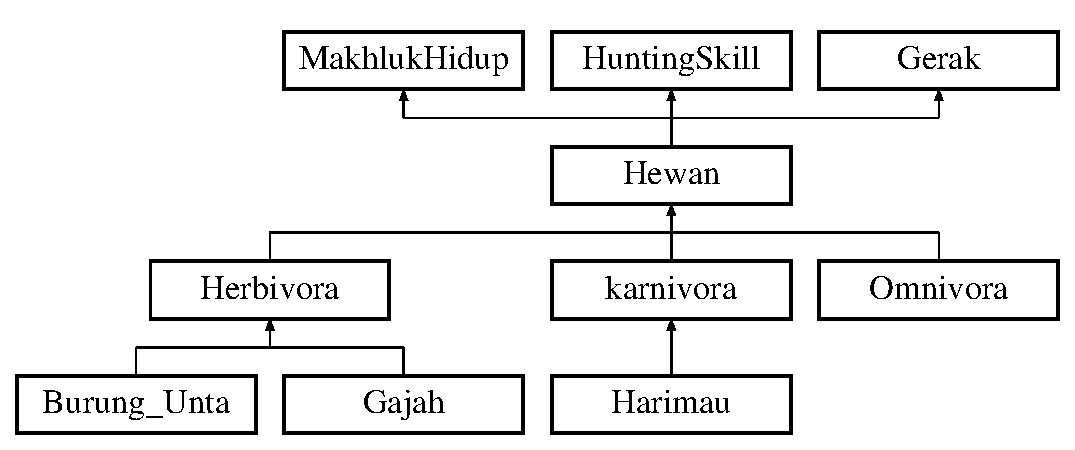
\includegraphics[height=3.733333cm]{class_hewan}
\end{center}
\end{figure}
\subsection*{Public Member Functions}
\begin{DoxyCompactItemize}
\item 
\hyperlink{class_hewan_a6b148b7d2380f746f2c7943d9adc4e15}{Hewan} (int \+\_\+umur=0, char \+\_\+\+D\+NA= \textquotesingle{}$\ast$\textquotesingle{}, int \+\_\+ulangtahun=0, \hyperlink{class_point}{Point} P=P\+Awal, int kenyang=0, int maks=0, char $\ast$tar=N\+U\+LL, bool \+\_\+memburu=false, int k=0, int a=0)
\item 
\hyperlink{class_hewan_a9a7e8b448780d0ebff93d06d82c77795}{Hewan} (const \hyperlink{class_hewan}{Hewan} \&)
\item 
\hyperlink{class_hewan}{Hewan} \& \hyperlink{class_hewan_ae6fca2e8de85c914a6ac040a9aea3d58}{operator=} (const \hyperlink{class_hewan}{Hewan} \&)
\item 
void \hyperlink{class_hewan_a488b6dde625a4b75f0014856ce5f7a47}{set\+Lapar} ()
\item 
virtual \hyperlink{class_hewan_aa3bee8976cb61cae94ee920fc371cf6c}{$\sim$\+Hewan} ()
\item 
void \hyperlink{class_hewan_a54587f410e4a417aa48baad66e3abeab}{set\+\_\+tingkat\+\_\+kekenyangan} (int kenyang)
\item 
void \hyperlink{class_hewan_aff60666bdcd276a6d5538905e8132a8e}{set\+\_\+maks\+\_\+tingkat\+\_\+kekenyangan} (int maks)
\item 
int \hyperlink{class_hewan_abf1d8353674e5f68018a68f17804ea96}{get\+\_\+tingkat\+\_\+kekenyangan} ()
\item 
int \hyperlink{class_hewan_ac8d2313e06af76164b7ce143489596f7}{get\+\_\+maks\+\_\+tingkat\+\_\+kekenyangan} ()
\item 
bool \hyperlink{class_hewan_a79068d1eb649c561b12a92a5de159601}{get\+\_\+lapar} ()
\item 
void \hyperlink{class_hewan_a2a5a54ebd082dbbd8b3ccee27c8233c1}{hewan\+Mati} ()
\item 
void \hyperlink{class_hewan_a9e143b9a009a9c6931c5186fd6a01733}{gerak\+\_\+bebas} ()
\item 
void \hyperlink{class_hewan_a60d1ecc64ab1715a53c6b925046ef389}{gerak\+\_\+memburu} (\hyperlink{class_point}{Point} Target)
\item 
void \hyperlink{class_hewan_aad665dcba615fccf92e06b295e47c50a}{gerak\+\_\+berarah} ()
\end{DoxyCompactItemize}


\subsection{Detailed Description}
A \hyperlink{class_hewan}{Hewan} class. A Class that describe a \hyperlink{class_hewan}{Hewan}. 

\subsection{Constructor \& Destructor Documentation}
\index{Hewan@{Hewan}!Hewan@{Hewan}}
\index{Hewan@{Hewan}!Hewan@{Hewan}}
\subsubsection[{\texorpdfstring{Hewan(int \+\_\+umur=0, char \+\_\+\+D\+N\+A= \textquotesingle{}$\ast$\textquotesingle{}, int \+\_\+ulangtahun=0, Point P=\+P\+Awal, int kenyang=0, int maks=0, char $\ast$tar=\+N\+U\+L\+L, bool \+\_\+memburu=false, int k=0, int a=0)}{Hewan(int _umur=0, char _DNA= '*', int _ulangtahun=0, Point P=PAwal, int kenyang=0, int maks=0, char *tar=NULL, bool _memburu=false, int k=0, int a=0)}}]{\setlength{\rightskip}{0pt plus 5cm}Hewan\+::\+Hewan (
\begin{DoxyParamCaption}
\item[{int}]{\+\_\+umur = {\ttfamily 0}, }
\item[{char}]{\+\_\+\+D\+NA = {\ttfamily \textquotesingle{}$\ast$\textquotesingle{}}, }
\item[{int}]{\+\_\+ulangtahun = {\ttfamily 0}, }
\item[{{\bf Point}}]{P = {\ttfamily PAwal}, }
\item[{int}]{kenyang = {\ttfamily 0}, }
\item[{int}]{maks = {\ttfamily 0}, }
\item[{char $\ast$}]{tar = {\ttfamily NULL}, }
\item[{bool}]{\+\_\+memburu = {\ttfamily false}, }
\item[{int}]{k = {\ttfamily 0}, }
\item[{int}]{a = {\ttfamily 0}}
\end{DoxyParamCaption}
)}\hypertarget{class_hewan_a6b148b7d2380f746f2c7943d9adc4e15}{}\label{class_hewan_a6b148b7d2380f746f2c7943d9adc4e15}
A constructor Making an organism with a default value in every parameter \index{Hewan@{Hewan}!Hewan@{Hewan}}
\index{Hewan@{Hewan}!Hewan@{Hewan}}
\subsubsection[{\texorpdfstring{Hewan(const Hewan \&)}{Hewan(const Hewan &)}}]{\setlength{\rightskip}{0pt plus 5cm}Hewan\+::\+Hewan (
\begin{DoxyParamCaption}
\item[{const {\bf Hewan} \&}]{H}
\end{DoxyParamCaption}
)}\hypertarget{class_hewan_a9a7e8b448780d0ebff93d06d82c77795}{}\label{class_hewan_a9a7e8b448780d0ebff93d06d82c77795}
A copy constructor \index{Hewan@{Hewan}!````~Hewan@{$\sim$\+Hewan}}
\index{````~Hewan@{$\sim$\+Hewan}!Hewan@{Hewan}}
\subsubsection[{\texorpdfstring{$\sim$\+Hewan()}{~Hewan()}}]{\setlength{\rightskip}{0pt plus 5cm}Hewan\+::$\sim$\+Hewan (
\begin{DoxyParamCaption}
{}
\end{DoxyParamCaption}
)\hspace{0.3cm}{\ttfamily [virtual]}}\hypertarget{class_hewan_aa3bee8976cb61cae94ee920fc371cf6c}{}\label{class_hewan_aa3bee8976cb61cae94ee920fc371cf6c}
A destructor Virtual destructor to destruct an organism 

\subsection{Member Function Documentation}
\index{Hewan@{Hewan}!gerak\+\_\+bebas@{gerak\+\_\+bebas}}
\index{gerak\+\_\+bebas@{gerak\+\_\+bebas}!Hewan@{Hewan}}
\subsubsection[{\texorpdfstring{gerak\+\_\+bebas()}{gerak_bebas()}}]{\setlength{\rightskip}{0pt plus 5cm}void Hewan\+::gerak\+\_\+bebas (
\begin{DoxyParamCaption}
{}
\end{DoxyParamCaption}
)}\hypertarget{class_hewan_a9e143b9a009a9c6931c5186fd6a01733}{}\label{class_hewan_a9e143b9a009a9c6931c5186fd6a01733}
A normal procedure member A procedure that makes animal move freely \index{Hewan@{Hewan}!gerak\+\_\+berarah@{gerak\+\_\+berarah}}
\index{gerak\+\_\+berarah@{gerak\+\_\+berarah}!Hewan@{Hewan}}
\subsubsection[{\texorpdfstring{gerak\+\_\+berarah()}{gerak_berarah()}}]{\setlength{\rightskip}{0pt plus 5cm}void Hewan\+::gerak\+\_\+berarah (
\begin{DoxyParamCaption}
{}
\end{DoxyParamCaption}
)}\hypertarget{class_hewan_aad665dcba615fccf92e06b295e47c50a}{}\label{class_hewan_aad665dcba615fccf92e06b295e47c50a}
A normal procedure member A procedure that makes animal move in a direction that has been set \index{Hewan@{Hewan}!gerak\+\_\+memburu@{gerak\+\_\+memburu}}
\index{gerak\+\_\+memburu@{gerak\+\_\+memburu}!Hewan@{Hewan}}
\subsubsection[{\texorpdfstring{gerak\+\_\+memburu(\+Point Target)}{gerak_memburu(Point Target)}}]{\setlength{\rightskip}{0pt plus 5cm}void Hewan\+::gerak\+\_\+memburu (
\begin{DoxyParamCaption}
\item[{{\bf Point}}]{Target}
\end{DoxyParamCaption}
)}\hypertarget{class_hewan_a60d1ecc64ab1715a53c6b925046ef389}{}\label{class_hewan_a60d1ecc64ab1715a53c6b925046ef389}
A normal procedure member that take one argument 
\begin{DoxyParams}{Parameters}
{\em A} & \hyperlink{class_point}{Point} of the target A procedure that makes the animal hunting the target \\
\hline
\end{DoxyParams}
\index{Hewan@{Hewan}!get\+\_\+lapar@{get\+\_\+lapar}}
\index{get\+\_\+lapar@{get\+\_\+lapar}!Hewan@{Hewan}}
\subsubsection[{\texorpdfstring{get\+\_\+lapar()}{get_lapar()}}]{\setlength{\rightskip}{0pt plus 5cm}bool Hewan\+::get\+\_\+lapar (
\begin{DoxyParamCaption}
{}
\end{DoxyParamCaption}
)}\hypertarget{class_hewan_a79068d1eb649c561b12a92a5de159601}{}\label{class_hewan_a79068d1eb649c561b12a92a5de159601}
A getter for hunger status \begin{DoxyReturn}{Returns}
a boolean 
\end{DoxyReturn}
\index{Hewan@{Hewan}!get\+\_\+maks\+\_\+tingkat\+\_\+kekenyangan@{get\+\_\+maks\+\_\+tingkat\+\_\+kekenyangan}}
\index{get\+\_\+maks\+\_\+tingkat\+\_\+kekenyangan@{get\+\_\+maks\+\_\+tingkat\+\_\+kekenyangan}!Hewan@{Hewan}}
\subsubsection[{\texorpdfstring{get\+\_\+maks\+\_\+tingkat\+\_\+kekenyangan()}{get_maks_tingkat_kekenyangan()}}]{\setlength{\rightskip}{0pt plus 5cm}int Hewan\+::get\+\_\+maks\+\_\+tingkat\+\_\+kekenyangan (
\begin{DoxyParamCaption}
{}
\end{DoxyParamCaption}
)}\hypertarget{class_hewan_ac8d2313e06af76164b7ce143489596f7}{}\label{class_hewan_ac8d2313e06af76164b7ce143489596f7}
A getter for maks\+\_\+tingkat\+\_\+kekenyangan \begin{DoxyReturn}{Returns}
an integer 
\end{DoxyReturn}
\index{Hewan@{Hewan}!get\+\_\+tingkat\+\_\+kekenyangan@{get\+\_\+tingkat\+\_\+kekenyangan}}
\index{get\+\_\+tingkat\+\_\+kekenyangan@{get\+\_\+tingkat\+\_\+kekenyangan}!Hewan@{Hewan}}
\subsubsection[{\texorpdfstring{get\+\_\+tingkat\+\_\+kekenyangan()}{get_tingkat_kekenyangan()}}]{\setlength{\rightskip}{0pt plus 5cm}int Hewan\+::get\+\_\+tingkat\+\_\+kekenyangan (
\begin{DoxyParamCaption}
{}
\end{DoxyParamCaption}
)}\hypertarget{class_hewan_abf1d8353674e5f68018a68f17804ea96}{}\label{class_hewan_abf1d8353674e5f68018a68f17804ea96}
A getter for tingkat\+\_\+kekenyangan \begin{DoxyReturn}{Returns}
an integer 
\end{DoxyReturn}
\index{Hewan@{Hewan}!hewan\+Mati@{hewan\+Mati}}
\index{hewan\+Mati@{hewan\+Mati}!Hewan@{Hewan}}
\subsubsection[{\texorpdfstring{hewan\+Mati()}{hewanMati()}}]{\setlength{\rightskip}{0pt plus 5cm}void Hewan\+::hewan\+Mati (
\begin{DoxyParamCaption}
{}
\end{DoxyParamCaption}
)}\hypertarget{class_hewan_a2a5a54ebd082dbbd8b3ccee27c8233c1}{}\label{class_hewan_a2a5a54ebd082dbbd8b3ccee27c8233c1}
A normal procedure member A procedure that processing the death of the animal \index{Hewan@{Hewan}!operator=@{operator=}}
\index{operator=@{operator=}!Hewan@{Hewan}}
\subsubsection[{\texorpdfstring{operator=(const Hewan \&)}{operator=(const Hewan &)}}]{\setlength{\rightskip}{0pt plus 5cm}{\bf Hewan} \& Hewan\+::operator= (
\begin{DoxyParamCaption}
\item[{const {\bf Hewan} \&}]{H}
\end{DoxyParamCaption}
)}\hypertarget{class_hewan_ae6fca2e8de85c914a6ac040a9aea3d58}{}\label{class_hewan_ae6fca2e8de85c914a6ac040a9aea3d58}
An operator = \index{Hewan@{Hewan}!set\+\_\+maks\+\_\+tingkat\+\_\+kekenyangan@{set\+\_\+maks\+\_\+tingkat\+\_\+kekenyangan}}
\index{set\+\_\+maks\+\_\+tingkat\+\_\+kekenyangan@{set\+\_\+maks\+\_\+tingkat\+\_\+kekenyangan}!Hewan@{Hewan}}
\subsubsection[{\texorpdfstring{set\+\_\+maks\+\_\+tingkat\+\_\+kekenyangan(int maks)}{set_maks_tingkat_kekenyangan(int maks)}}]{\setlength{\rightskip}{0pt plus 5cm}void Hewan\+::set\+\_\+maks\+\_\+tingkat\+\_\+kekenyangan (
\begin{DoxyParamCaption}
\item[{int}]{maks}
\end{DoxyParamCaption}
)}\hypertarget{class_hewan_aff60666bdcd276a6d5538905e8132a8e}{}\label{class_hewan_aff60666bdcd276a6d5538905e8132a8e}
A setter for maks\+\_\+tingkat\+\_\+kekenyangan 
\begin{DoxyParams}{Parameters}
{\em an} & integer arguments that will be assigned to maks\+\_\+tingkat\+\_\+kekenyangan \\
\hline
\end{DoxyParams}
\index{Hewan@{Hewan}!set\+\_\+tingkat\+\_\+kekenyangan@{set\+\_\+tingkat\+\_\+kekenyangan}}
\index{set\+\_\+tingkat\+\_\+kekenyangan@{set\+\_\+tingkat\+\_\+kekenyangan}!Hewan@{Hewan}}
\subsubsection[{\texorpdfstring{set\+\_\+tingkat\+\_\+kekenyangan(int kenyang)}{set_tingkat_kekenyangan(int kenyang)}}]{\setlength{\rightskip}{0pt plus 5cm}void Hewan\+::set\+\_\+tingkat\+\_\+kekenyangan (
\begin{DoxyParamCaption}
\item[{int}]{kenyang}
\end{DoxyParamCaption}
)}\hypertarget{class_hewan_a54587f410e4a417aa48baad66e3abeab}{}\label{class_hewan_a54587f410e4a417aa48baad66e3abeab}
A setter for tingkat\+\_\+kekenyangan 
\begin{DoxyParams}{Parameters}
{\em an} & integer arguments that will be assigned to tingkat\+\_\+kekenyangan \\
\hline
\end{DoxyParams}
\index{Hewan@{Hewan}!set\+Lapar@{set\+Lapar}}
\index{set\+Lapar@{set\+Lapar}!Hewan@{Hewan}}
\subsubsection[{\texorpdfstring{set\+Lapar()}{setLapar()}}]{\setlength{\rightskip}{0pt plus 5cm}void Hewan\+::set\+Lapar (
\begin{DoxyParamCaption}
{}
\end{DoxyParamCaption}
)}\hypertarget{class_hewan_a488b6dde625a4b75f0014856ce5f7a47}{}\label{class_hewan_a488b6dde625a4b75f0014856ce5f7a47}
A normal procedure member A procedure that set the hunger status of the organism 

The documentation for this class was generated from the following files\+:\begin{DoxyCompactItemize}
\item 
Hewan.\+h\item 
Hewan.\+cpp\end{DoxyCompactItemize}

\hypertarget{class_hunting_skill}{}\section{Hunting\+Skill Class Reference}
\label{class_hunting_skill}\index{Hunting\+Skill@{Hunting\+Skill}}
Inheritance diagram for Hunting\+Skill\+:\begin{figure}[H]
\begin{center}
\leavevmode
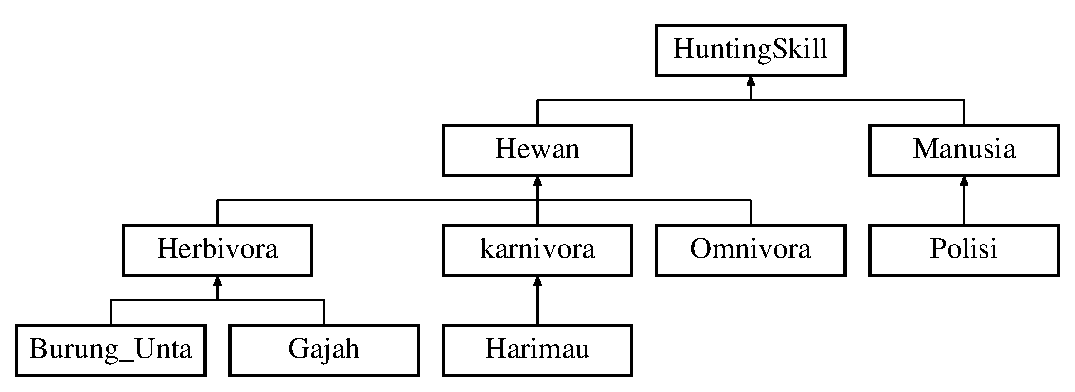
\includegraphics[height=4.000000cm]{class_hunting_skill}
\end{center}
\end{figure}
\subsection*{Public Member Functions}
\begin{DoxyCompactItemize}
\item 
{\bfseries Hunting\+Skill} (char $\ast$Target=N\+U\+LL)\hypertarget{class_hunting_skill_abca94691ed5e1dd038ce02a70e71254d}{}\label{class_hunting_skill_abca94691ed5e1dd038ce02a70e71254d}

\item 
{\bfseries Hunting\+Skill} (const \hyperlink{class_hunting_skill}{Hunting\+Skill} \&)\hypertarget{class_hunting_skill_a8817bc85912e00b4b431a94f32ee494e}{}\label{class_hunting_skill_a8817bc85912e00b4b431a94f32ee494e}

\item 
\hyperlink{class_hunting_skill}{Hunting\+Skill} \& {\bfseries operator=} (const \hyperlink{class_hunting_skill}{Hunting\+Skill} \&)\hypertarget{class_hunting_skill_abd3b1e20a12499d97eb24f428be09d2d}{}\label{class_hunting_skill_abd3b1e20a12499d97eb24f428be09d2d}

\item 
void {\bfseries set\+Memburu} (bool M)\hypertarget{class_hunting_skill_a9e00e9c4f2548ab4d25acb513625e364}{}\label{class_hunting_skill_a9e00e9c4f2548ab4d25acb513625e364}

\item 
char $\ast$ {\bfseries get\+Target} ()\hypertarget{class_hunting_skill_ace96396eca2bb39cddd326c2dc22243c}{}\label{class_hunting_skill_ace96396eca2bb39cddd326c2dc22243c}

\item 
bool {\bfseries get\+Memburu} ()\hypertarget{class_hunting_skill_a1556fa4584ab19e2887e448fe5f6d34f}{}\label{class_hunting_skill_a1556fa4584ab19e2887e448fe5f6d34f}

\end{DoxyCompactItemize}


The documentation for this class was generated from the following files\+:\begin{DoxyCompactItemize}
\item 
C\+:/\+Users/\+C\+X\+X\+X\+V/\+Documents/\+Git\+Hub/\+Makhluk/Hunting\+Skill.\+h\item 
C\+:/\+Users/\+C\+X\+X\+X\+V/\+Documents/\+Git\+Hub/\+Makhluk/Hunting\+Skill.\+cpp\end{DoxyCompactItemize}

\hypertarget{classkarnivora}{}\section{karnivora Class Reference}
\label{classkarnivora}\index{karnivora@{karnivora}}
Inheritance diagram for karnivora\+:\begin{figure}[H]
\begin{center}
\leavevmode
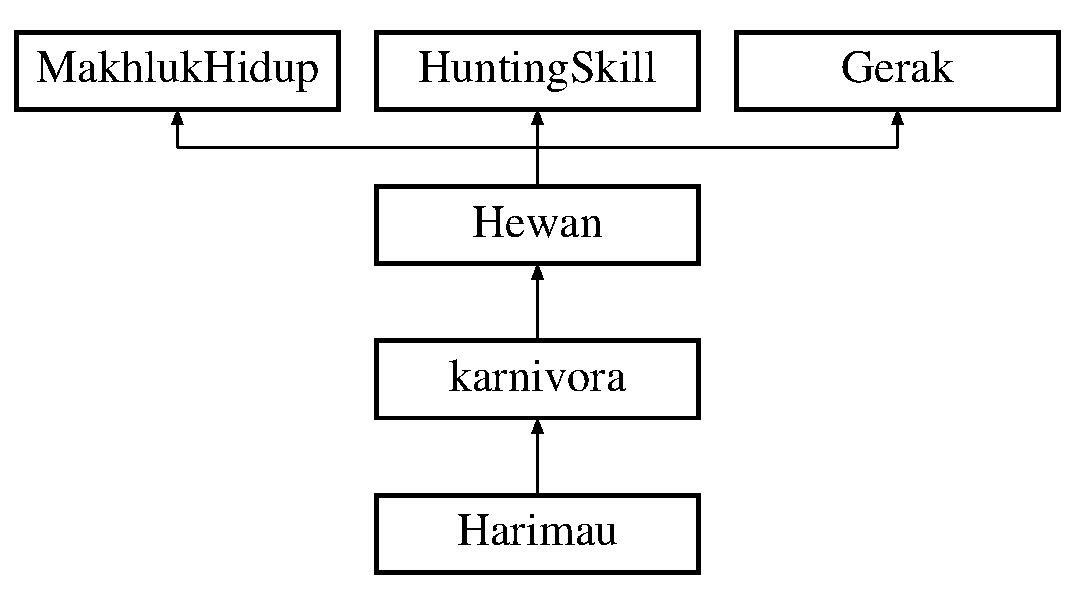
\includegraphics[height=4.000000cm]{classkarnivora}
\end{center}
\end{figure}
\subsection*{Public Member Functions}
\begin{DoxyCompactItemize}
\item 
virtual bool {\bfseries melambat} ()=0\hypertarget{classkarnivora_a94ff5f34e424327e3b6114fa69d519d1}{}\label{classkarnivora_a94ff5f34e424327e3b6114fa69d519d1}

\end{DoxyCompactItemize}
\subsection*{Protected Attributes}
\begin{DoxyCompactItemize}
\item 
int {\bfseries delta\+Kecepatan}\hypertarget{classkarnivora_af4eecf0a583853a91f8b26f153b4f97a}{}\label{classkarnivora_af4eecf0a583853a91f8b26f153b4f97a}

\end{DoxyCompactItemize}


The documentation for this class was generated from the following file\+:\begin{DoxyCompactItemize}
\item 
C\+:/\+Users/\+C\+X\+X\+X\+V/\+Documents/\+Git\+Hub/\+Makhluk/Karnivora.\+h\end{DoxyCompactItemize}

\hypertarget{class_konduktor_makhluk_hidup}{}\section{Konduktor\+Makhluk\+Hidup Class Reference}
\label{class_konduktor_makhluk_hidup}\index{Konduktor\+Makhluk\+Hidup@{Konduktor\+Makhluk\+Hidup}}


{\ttfamily \#include $<$konduktor\+Makhluk\+Hidup.\+h$>$}

Inheritance diagram for Konduktor\+Makhluk\+Hidup\+:\begin{figure}[H]
\begin{center}
\leavevmode
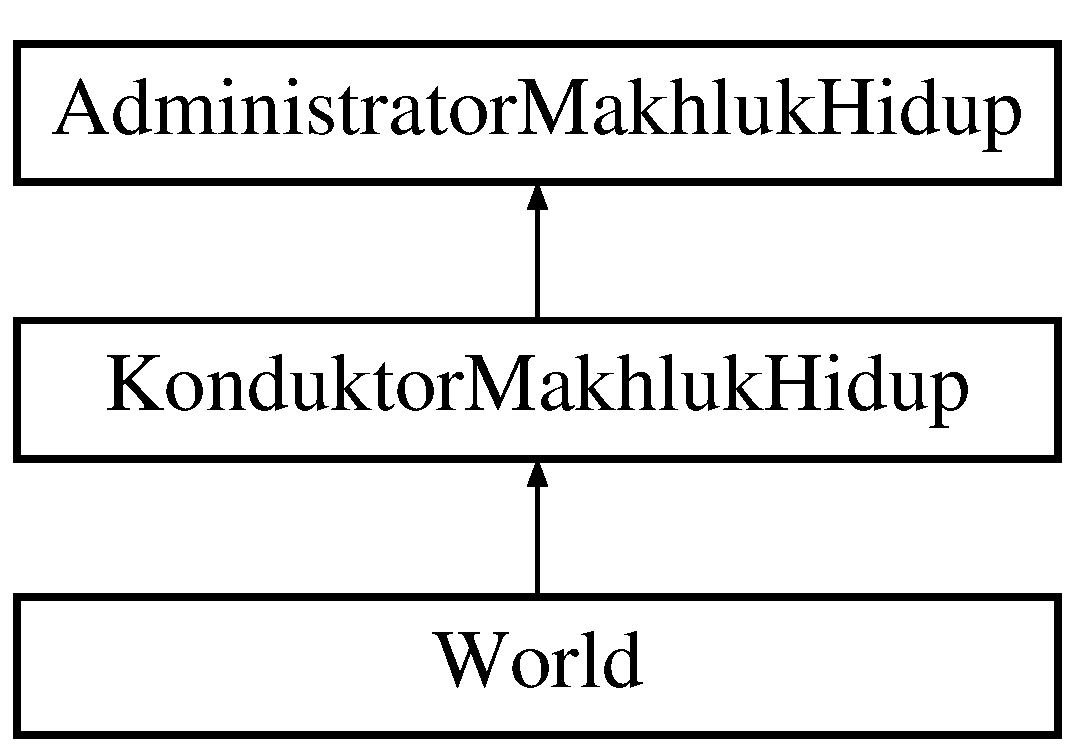
\includegraphics[height=2.000000cm]{class_konduktor_makhluk_hidup}
\end{center}
\end{figure}
\subsection*{Public Member Functions}
\begin{DoxyCompactItemize}
\item 
\hyperlink{class_konduktor_makhluk_hidup_a2b85d7afd1474acec8d394a5e10cecd6}{Konduktor\+Makhluk\+Hidup} ()
\item 
void \hyperlink{class_konduktor_makhluk_hidup_a87e20c1fac7f69730e1f800928fdab59}{hidup} (\hyperlink{class_manusia}{Manusia} \&)
\item 
void \hyperlink{class_konduktor_makhluk_hidup_a6db50a642d5f184ca11aaeb6e275797f}{hidup} (\hyperlink{class_herbivora}{Herbivora} \&)
\item 
void \hyperlink{class_konduktor_makhluk_hidup_a46e2bf54054641c6c8b377ef4052da39}{hidup} (\hyperlink{class_karnivora}{Karnivora} \&)
\item 
void \hyperlink{class_konduktor_makhluk_hidup_a54ce9beb02fffa0320fd8f8a1315e255}{hidup} (\hyperlink{class_omnivora}{Omnivora} \&)
\item 
void \hyperlink{class_konduktor_makhluk_hidup_a247cde5e3f3e8bf9ffa015b90e29fe38}{hidup} (\hyperlink{class_tumbuhan}{Tumbuhan} \&)
\item 
void \hyperlink{class_konduktor_makhluk_hidup_a90086da731ab404c57c96db90d6bb968}{pause} ()
\item 
void \hyperlink{class_konduktor_makhluk_hidup_af1086cb49d657605bb998db36abec897}{resume} ()
\item 
void \hyperlink{class_konduktor_makhluk_hidup_aa241caf5c346f96f9717183dd60b9414}{aging} (\hyperlink{class_makhluk_hidup}{Makhluk\+Hidup} \&)
\item 
void \hyperlink{class_konduktor_makhluk_hidup_aa299db55a0e7ab426d2ba61bda3b84a5}{set\+Bawah} (int)
\item 
void \hyperlink{class_konduktor_makhluk_hidup_aa120358e949c0dc53286cbff0d5ea4e3}{set\+Samping} (int)
\item 
int \hyperlink{class_konduktor_makhluk_hidup_a4c9b65dc15d4b3b3a41b885b5030009c}{Get\+Bawah} ()
\item 
int \hyperlink{class_konduktor_makhluk_hidup_a453d35d38b281010dead4ea842be9360}{Get\+Samping} ()
\end{DoxyCompactItemize}


\subsection{Detailed Description}
A class to control a \hyperlink{class_makhluk_hidup}{Makhluk\+Hidup} 

\subsection{Constructor \& Destructor Documentation}
\index{Konduktor\+Makhluk\+Hidup@{Konduktor\+Makhluk\+Hidup}!Konduktor\+Makhluk\+Hidup@{Konduktor\+Makhluk\+Hidup}}
\index{Konduktor\+Makhluk\+Hidup@{Konduktor\+Makhluk\+Hidup}!Konduktor\+Makhluk\+Hidup@{Konduktor\+Makhluk\+Hidup}}
\subsubsection[{\texorpdfstring{Konduktor\+Makhluk\+Hidup()}{KonduktorMakhlukHidup()}}]{\setlength{\rightskip}{0pt plus 5cm}Konduktor\+Makhluk\+Hidup\+::\+Konduktor\+Makhluk\+Hidup (
\begin{DoxyParamCaption}
{}
\end{DoxyParamCaption}
)}\hypertarget{class_konduktor_makhluk_hidup_a2b85d7afd1474acec8d394a5e10cecd6}{}\label{class_konduktor_makhluk_hidup_a2b85d7afd1474acec8d394a5e10cecd6}
ctor which initialize lifestate with 1 

\subsection{Member Function Documentation}
\index{Konduktor\+Makhluk\+Hidup@{Konduktor\+Makhluk\+Hidup}!aging@{aging}}
\index{aging@{aging}!Konduktor\+Makhluk\+Hidup@{Konduktor\+Makhluk\+Hidup}}
\subsubsection[{\texorpdfstring{aging(\+Makhluk\+Hidup \&)}{aging(MakhlukHidup &)}}]{\setlength{\rightskip}{0pt plus 5cm}void Konduktor\+Makhluk\+Hidup\+::aging (
\begin{DoxyParamCaption}
\item[{{\bf Makhluk\+Hidup} \&}]{m1}
\end{DoxyParamCaption}
)}\hypertarget{class_konduktor_makhluk_hidup_aa241caf5c346f96f9717183dd60b9414}{}\label{class_konduktor_makhluk_hidup_aa241caf5c346f96f9717183dd60b9414}
Increase the umur of a \hyperlink{class_makhluk_hidup}{Makhluk\+Hidup} 
\begin{DoxyParams}{Parameters}
{\em a} & \hyperlink{class_makhluk_hidup}{Makhluk\+Hidup} \\
\hline
\end{DoxyParams}
\index{Konduktor\+Makhluk\+Hidup@{Konduktor\+Makhluk\+Hidup}!Get\+Bawah@{Get\+Bawah}}
\index{Get\+Bawah@{Get\+Bawah}!Konduktor\+Makhluk\+Hidup@{Konduktor\+Makhluk\+Hidup}}
\subsubsection[{\texorpdfstring{Get\+Bawah()}{GetBawah()}}]{\setlength{\rightskip}{0pt plus 5cm}int Konduktor\+Makhluk\+Hidup\+::\+Get\+Bawah (
\begin{DoxyParamCaption}
{}
\end{DoxyParamCaption}
)}\hypertarget{class_konduktor_makhluk_hidup_a4c9b65dc15d4b3b3a41b885b5030009c}{}\label{class_konduktor_makhluk_hidup_a4c9b65dc15d4b3b3a41b885b5030009c}
returns the value of batas\+Bawah \begin{DoxyReturn}{Returns}
an integer 
\end{DoxyReturn}
\index{Konduktor\+Makhluk\+Hidup@{Konduktor\+Makhluk\+Hidup}!Get\+Samping@{Get\+Samping}}
\index{Get\+Samping@{Get\+Samping}!Konduktor\+Makhluk\+Hidup@{Konduktor\+Makhluk\+Hidup}}
\subsubsection[{\texorpdfstring{Get\+Samping()}{GetSamping()}}]{\setlength{\rightskip}{0pt plus 5cm}int Konduktor\+Makhluk\+Hidup\+::\+Get\+Samping (
\begin{DoxyParamCaption}
{}
\end{DoxyParamCaption}
)}\hypertarget{class_konduktor_makhluk_hidup_a453d35d38b281010dead4ea842be9360}{}\label{class_konduktor_makhluk_hidup_a453d35d38b281010dead4ea842be9360}
returns the value of batas\+Samping \begin{DoxyReturn}{Returns}
an integer 
\end{DoxyReturn}
\index{Konduktor\+Makhluk\+Hidup@{Konduktor\+Makhluk\+Hidup}!hidup@{hidup}}
\index{hidup@{hidup}!Konduktor\+Makhluk\+Hidup@{Konduktor\+Makhluk\+Hidup}}
\subsubsection[{\texorpdfstring{hidup(\+Manusia \&)}{hidup(Manusia &)}}]{\setlength{\rightskip}{0pt plus 5cm}void Konduktor\+Makhluk\+Hidup\+::hidup (
\begin{DoxyParamCaption}
\item[{{\bf Manusia} \&}]{m1}
\end{DoxyParamCaption}
)}\hypertarget{class_konduktor_makhluk_hidup_a87e20c1fac7f69730e1f800928fdab59}{}\label{class_konduktor_makhluk_hidup_a87e20c1fac7f69730e1f800928fdab59}
Told a \hyperlink{class_manusia}{Manusia} to do it\textquotesingle{}s behaviour 
\begin{DoxyParams}{Parameters}
{\em a} & \hyperlink{class_manusia}{Manusia} \\
\hline
\end{DoxyParams}
\index{Konduktor\+Makhluk\+Hidup@{Konduktor\+Makhluk\+Hidup}!hidup@{hidup}}
\index{hidup@{hidup}!Konduktor\+Makhluk\+Hidup@{Konduktor\+Makhluk\+Hidup}}
\subsubsection[{\texorpdfstring{hidup(\+Herbivora \&)}{hidup(Herbivora &)}}]{\setlength{\rightskip}{0pt plus 5cm}void Konduktor\+Makhluk\+Hidup\+::hidup (
\begin{DoxyParamCaption}
\item[{{\bf Herbivora} \&}]{m1}
\end{DoxyParamCaption}
)}\hypertarget{class_konduktor_makhluk_hidup_a6db50a642d5f184ca11aaeb6e275797f}{}\label{class_konduktor_makhluk_hidup_a6db50a642d5f184ca11aaeb6e275797f}
Told a \hyperlink{class_herbivora}{Herbivora} to do it\textquotesingle{}s behaviour 
\begin{DoxyParams}{Parameters}
{\em a} & Herbivore \\
\hline
\end{DoxyParams}
\index{Konduktor\+Makhluk\+Hidup@{Konduktor\+Makhluk\+Hidup}!hidup@{hidup}}
\index{hidup@{hidup}!Konduktor\+Makhluk\+Hidup@{Konduktor\+Makhluk\+Hidup}}
\subsubsection[{\texorpdfstring{hidup(\+Karnivora \&)}{hidup(Karnivora &)}}]{\setlength{\rightskip}{0pt plus 5cm}void Konduktor\+Makhluk\+Hidup\+::hidup (
\begin{DoxyParamCaption}
\item[{{\bf Karnivora} \&}]{m1}
\end{DoxyParamCaption}
)}\hypertarget{class_konduktor_makhluk_hidup_a46e2bf54054641c6c8b377ef4052da39}{}\label{class_konduktor_makhluk_hidup_a46e2bf54054641c6c8b377ef4052da39}
Told a \hyperlink{class_karnivora}{Karnivora} to do it\textquotesingle{}s behaviour 
\begin{DoxyParams}{Parameters}
{\em a} & \hyperlink{class_karnivora}{Karnivora} \\
\hline
\end{DoxyParams}
\index{Konduktor\+Makhluk\+Hidup@{Konduktor\+Makhluk\+Hidup}!hidup@{hidup}}
\index{hidup@{hidup}!Konduktor\+Makhluk\+Hidup@{Konduktor\+Makhluk\+Hidup}}
\subsubsection[{\texorpdfstring{hidup(\+Omnivora \&)}{hidup(Omnivora &)}}]{\setlength{\rightskip}{0pt plus 5cm}void Konduktor\+Makhluk\+Hidup\+::hidup (
\begin{DoxyParamCaption}
\item[{{\bf Omnivora} \&}]{m1}
\end{DoxyParamCaption}
)}\hypertarget{class_konduktor_makhluk_hidup_a54ce9beb02fffa0320fd8f8a1315e255}{}\label{class_konduktor_makhluk_hidup_a54ce9beb02fffa0320fd8f8a1315e255}
Told a \hyperlink{class_omnivora}{Omnivora} to do it\textquotesingle{}s behaviour 
\begin{DoxyParams}{Parameters}
{\em a} & \hyperlink{class_omnivora}{Omnivora} \\
\hline
\end{DoxyParams}
\index{Konduktor\+Makhluk\+Hidup@{Konduktor\+Makhluk\+Hidup}!hidup@{hidup}}
\index{hidup@{hidup}!Konduktor\+Makhluk\+Hidup@{Konduktor\+Makhluk\+Hidup}}
\subsubsection[{\texorpdfstring{hidup(\+Tumbuhan \&)}{hidup(Tumbuhan &)}}]{\setlength{\rightskip}{0pt plus 5cm}void Konduktor\+Makhluk\+Hidup\+::hidup (
\begin{DoxyParamCaption}
\item[{{\bf Tumbuhan} \&}]{t1}
\end{DoxyParamCaption}
)}\hypertarget{class_konduktor_makhluk_hidup_a247cde5e3f3e8bf9ffa015b90e29fe38}{}\label{class_konduktor_makhluk_hidup_a247cde5e3f3e8bf9ffa015b90e29fe38}
Told a \hyperlink{class_tumbuhan}{Tumbuhan} to do it\textquotesingle{}s behaviour 
\begin{DoxyParams}{Parameters}
{\em a} & \hyperlink{class_tumbuhan}{Tumbuhan} \\
\hline
\end{DoxyParams}
\index{Konduktor\+Makhluk\+Hidup@{Konduktor\+Makhluk\+Hidup}!pause@{pause}}
\index{pause@{pause}!Konduktor\+Makhluk\+Hidup@{Konduktor\+Makhluk\+Hidup}}
\subsubsection[{\texorpdfstring{pause()}{pause()}}]{\setlength{\rightskip}{0pt plus 5cm}void Konduktor\+Makhluk\+Hidup\+::pause (
\begin{DoxyParamCaption}
{}
\end{DoxyParamCaption}
)}\hypertarget{class_konduktor_makhluk_hidup_a90086da731ab404c57c96db90d6bb968}{}\label{class_konduktor_makhluk_hidup_a90086da731ab404c57c96db90d6bb968}
prevent all behavior to be done \index{Konduktor\+Makhluk\+Hidup@{Konduktor\+Makhluk\+Hidup}!resume@{resume}}
\index{resume@{resume}!Konduktor\+Makhluk\+Hidup@{Konduktor\+Makhluk\+Hidup}}
\subsubsection[{\texorpdfstring{resume()}{resume()}}]{\setlength{\rightskip}{0pt plus 5cm}void Konduktor\+Makhluk\+Hidup\+::resume (
\begin{DoxyParamCaption}
{}
\end{DoxyParamCaption}
)}\hypertarget{class_konduktor_makhluk_hidup_af1086cb49d657605bb998db36abec897}{}\label{class_konduktor_makhluk_hidup_af1086cb49d657605bb998db36abec897}
cancel a pause \index{Konduktor\+Makhluk\+Hidup@{Konduktor\+Makhluk\+Hidup}!set\+Bawah@{set\+Bawah}}
\index{set\+Bawah@{set\+Bawah}!Konduktor\+Makhluk\+Hidup@{Konduktor\+Makhluk\+Hidup}}
\subsubsection[{\texorpdfstring{set\+Bawah(int)}{setBawah(int)}}]{\setlength{\rightskip}{0pt plus 5cm}void Konduktor\+Makhluk\+Hidup\+::set\+Bawah (
\begin{DoxyParamCaption}
\item[{int}]{i}
\end{DoxyParamCaption}
)}\hypertarget{class_konduktor_makhluk_hidup_aa299db55a0e7ab426d2ba61bda3b84a5}{}\label{class_konduktor_makhluk_hidup_aa299db55a0e7ab426d2ba61bda3b84a5}
Set the value of batas\+Bawah 
\begin{DoxyParams}{Parameters}
{\em an} & integer \\
\hline
\end{DoxyParams}
\index{Konduktor\+Makhluk\+Hidup@{Konduktor\+Makhluk\+Hidup}!set\+Samping@{set\+Samping}}
\index{set\+Samping@{set\+Samping}!Konduktor\+Makhluk\+Hidup@{Konduktor\+Makhluk\+Hidup}}
\subsubsection[{\texorpdfstring{set\+Samping(int)}{setSamping(int)}}]{\setlength{\rightskip}{0pt plus 5cm}void Konduktor\+Makhluk\+Hidup\+::set\+Samping (
\begin{DoxyParamCaption}
\item[{int}]{i}
\end{DoxyParamCaption}
)}\hypertarget{class_konduktor_makhluk_hidup_aa120358e949c0dc53286cbff0d5ea4e3}{}\label{class_konduktor_makhluk_hidup_aa120358e949c0dc53286cbff0d5ea4e3}
Set the value of batas\+Samping 
\begin{DoxyParams}{Parameters}
{\em an} & integer \\
\hline
\end{DoxyParams}


The documentation for this class was generated from the following files\+:\begin{DoxyCompactItemize}
\item 
konduktor\+Makhluk\+Hidup.\+h\item 
konduktor\+Makhluk\+Hidup.\+cpp\end{DoxyCompactItemize}

\hypertarget{class_makhluk_hidup}{}\section{Makhluk\+Hidup Class Reference}
\label{class_makhluk_hidup}\index{Makhluk\+Hidup@{Makhluk\+Hidup}}
Inheritance diagram for Makhluk\+Hidup\+:\begin{figure}[H]
\begin{center}
\leavevmode
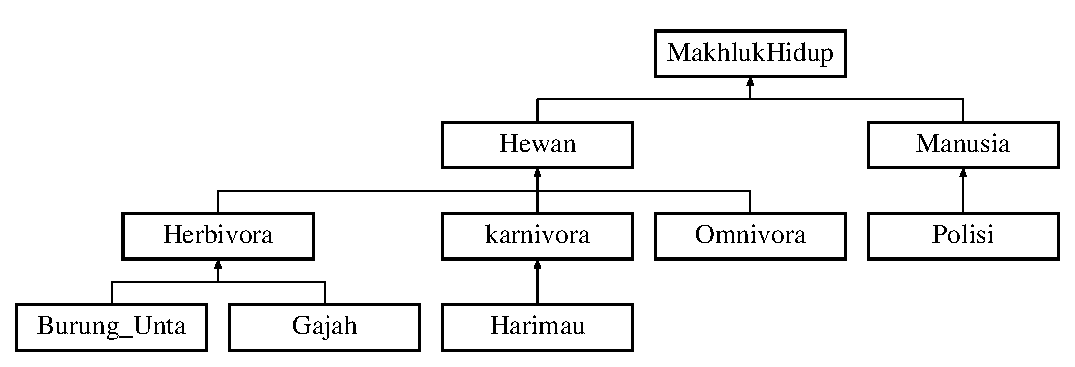
\includegraphics[height=4.000000cm]{class_makhluk_hidup}
\end{center}
\end{figure}
\subsection*{Public Member Functions}
\begin{DoxyCompactItemize}
\item 
{\bfseries Makhluk\+Hidup} (int \+\_\+umur=0, char \+\_\+\+D\+NA= \textquotesingle{}$\ast$\textquotesingle{}, int \+\_\+ulangtahun=0, \hyperlink{class_point}{Point} P=P\+Awal)\hypertarget{class_makhluk_hidup_aa2b7d6507df43a37523592ae194cc30f}{}\label{class_makhluk_hidup_aa2b7d6507df43a37523592ae194cc30f}

\item 
{\bfseries Makhluk\+Hidup} (const \hyperlink{class_makhluk_hidup}{Makhluk\+Hidup} \&)\hypertarget{class_makhluk_hidup_ab4caed894c2ae2ab388ce59b0b5311d9}{}\label{class_makhluk_hidup_ab4caed894c2ae2ab388ce59b0b5311d9}

\item 
\hyperlink{class_makhluk_hidup}{Makhluk\+Hidup} \& {\bfseries operator=} (const \hyperlink{class_makhluk_hidup}{Makhluk\+Hidup} \&)\hypertarget{class_makhluk_hidup_a372abdbd24705c1edd3661436947fe22}{}\label{class_makhluk_hidup_a372abdbd24705c1edd3661436947fe22}

\item 
void {\bfseries menua} ()\hypertarget{class_makhluk_hidup_ae06db2e59854f4cd51aae77ea177405e}{}\label{class_makhluk_hidup_ae06db2e59854f4cd51aae77ea177405e}

\item 
bool {\bfseries mati} ()\hypertarget{class_makhluk_hidup_a5fe3d9e2262f499bbb1369cadf252d5c}{}\label{class_makhluk_hidup_a5fe3d9e2262f499bbb1369cadf252d5c}

\item 
void {\bfseries display} ()\hypertarget{class_makhluk_hidup_a5f680398fc4ad2f630b317695e9d4a4f}{}\label{class_makhluk_hidup_a5f680398fc4ad2f630b317695e9d4a4f}

\item 
int {\bfseries get\+\_\+umur} ()\hypertarget{class_makhluk_hidup_a05e688885d0a194c53412ef8c8f04890}{}\label{class_makhluk_hidup_a05e688885d0a194c53412ef8c8f04890}

\item 
int {\bfseries get\+\_\+ulang\+\_\+tahun} ()\hypertarget{class_makhluk_hidup_a4077d7a2a0f0a84858b15dadd181d945}{}\label{class_makhluk_hidup_a4077d7a2a0f0a84858b15dadd181d945}

\item 
char {\bfseries get\+\_\+\+D\+NA} ()\hypertarget{class_makhluk_hidup_a67f74ca50e81ff549d6b2c6a7cfcbba7}{}\label{class_makhluk_hidup_a67f74ca50e81ff549d6b2c6a7cfcbba7}

\item 
int {\bfseries get\+\_\+batas\+\_\+umur} ()\hypertarget{class_makhluk_hidup_a78cd2c91aba52d11f2e7606b52a706d4}{}\label{class_makhluk_hidup_a78cd2c91aba52d11f2e7606b52a706d4}

\item 
\hyperlink{class_point}{Point} {\bfseries get\+Posisi} ()\hypertarget{class_makhluk_hidup_a555874bb0b80f95157a7e2746ea36f35}{}\label{class_makhluk_hidup_a555874bb0b80f95157a7e2746ea36f35}

\item 
char {\bfseries get\+Predator} (int i)\hypertarget{class_makhluk_hidup_a97bc5cca37bfa18311e99ce63e39a009}{}\label{class_makhluk_hidup_a97bc5cca37bfa18311e99ce63e39a009}

\item 
int {\bfseries get\+Ukuran\+Predator} ()\hypertarget{class_makhluk_hidup_ad12076a7c63dde29e90b1f4ca48aaff1}{}\label{class_makhluk_hidup_ad12076a7c63dde29e90b1f4ca48aaff1}

\item 
void {\bfseries set\+\_\+umur} (int)\hypertarget{class_makhluk_hidup_adc7715c1915723fdf42ff205458923e7}{}\label{class_makhluk_hidup_adc7715c1915723fdf42ff205458923e7}

\item 
void {\bfseries set\+\_\+ulang\+\_\+tahun} (int)\hypertarget{class_makhluk_hidup_a9db02ead4d61096dbd8f7a9e26901e71}{}\label{class_makhluk_hidup_a9db02ead4d61096dbd8f7a9e26901e71}

\item 
void {\bfseries set\+\_\+\+D\+NA} (char)\hypertarget{class_makhluk_hidup_a816be4a8a08a2daccab170b99fb26ce9}{}\label{class_makhluk_hidup_a816be4a8a08a2daccab170b99fb26ce9}

\item 
void {\bfseries set\+Posisi} (\hyperlink{class_point}{Point})\hypertarget{class_makhluk_hidup_a62cb644f5defd2cc68783f52ef954b57}{}\label{class_makhluk_hidup_a62cb644f5defd2cc68783f52ef954b57}

\item 
void {\bfseries set\+Predator} (int i, char \+\_\+predator)\hypertarget{class_makhluk_hidup_add4f38ec95f2c1e5b715a7184105288a}{}\label{class_makhluk_hidup_add4f38ec95f2c1e5b715a7184105288a}

\end{DoxyCompactItemize}


The documentation for this class was generated from the following files\+:\begin{DoxyCompactItemize}
\item 
C\+:/\+Users/\+C\+X\+X\+X\+V/\+Documents/\+Git\+Hub/\+Makhluk/Makhluk\+Hidup.\+h\item 
C\+:/\+Users/\+C\+X\+X\+X\+V/\+Documents/\+Git\+Hub/\+Makhluk/Makhluk\+Hidup.\+cpp\end{DoxyCompactItemize}

\hypertarget{class_manusia}{}\section{Manusia Class Reference}
\label{class_manusia}\index{Manusia@{Manusia}}


{\ttfamily \#include $<$Manusia.\+h$>$}

Inheritance diagram for Manusia\+:\begin{figure}[H]
\begin{center}
\leavevmode
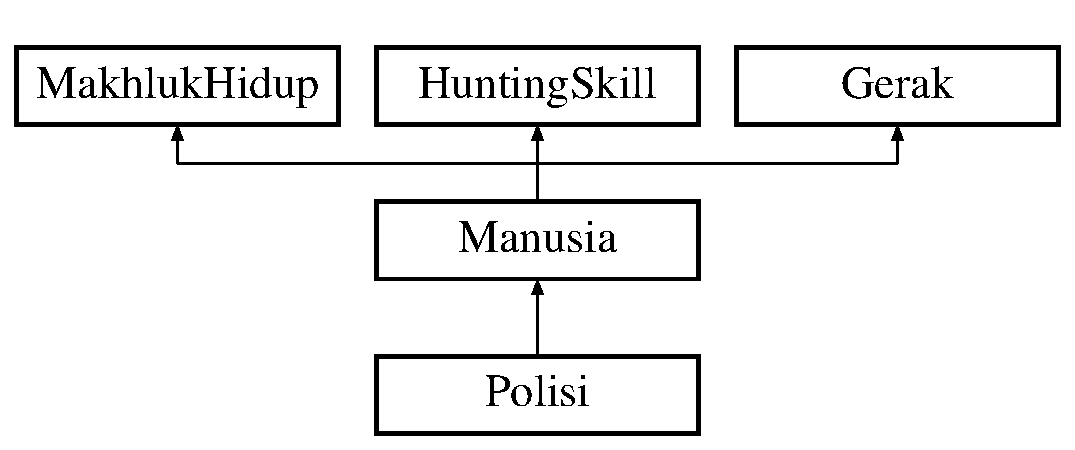
\includegraphics[height=3.000000cm]{class_manusia}
\end{center}
\end{figure}
\subsection*{Public Member Functions}
\begin{DoxyCompactItemize}
\item 
\hyperlink{class_manusia_a0fb22ce7d583e644cdaf1d426a2fca4f}{Manusia} (int \+\_\+umur=0, char \+\_\+\+D\+NA= \textquotesingle{}$\ast$\textquotesingle{}, int \+\_\+ulangtahun=0, \hyperlink{class_point}{Point} P=P\+Awal, char $\ast$Target=N\+U\+LL, bool \+\_\+memburu=false, int kec=0, int arah=0)
\item 
\hyperlink{class_manusia_ad575964df3ab12cae6e55c6f498e5739}{Manusia} (const \hyperlink{class_manusia}{Manusia} \&)
\item 
\hyperlink{class_manusia}{Manusia} \& \hyperlink{class_manusia_a5e450b3dde01ce84733c678346eb0caf}{operator=} (const \hyperlink{class_manusia}{Manusia} \&)
\item 
void \hyperlink{class_manusia_a0ad58fdb68abbcebaf7714d071e7e8d3}{set\+Menghindar} (bool m)
\item 
bool \hyperlink{class_manusia_a5606183ee0e8ad0c93a65a2cca6529a6}{get\+Menghindar} ()
\item 
void \hyperlink{class_manusia_a7f67dbd8c2c0bc8ce51d384f9c17746a}{gerak\+\_\+bebas} ()
\item 
void \hyperlink{class_manusia_aa4e3ef878fa2f00b5ca777d0386ae4c8}{gerak\+\_\+menjauh} (\hyperlink{class_point}{Point} Predator)
\item 
void \hyperlink{class_manusia_a090fe1eaf987dce764e219f06d922197}{gerak\+\_\+memburu} (\hyperlink{class_point}{Point} Target)
\item 
void \hyperlink{class_manusia_a636a0198adb7029b5c00ccee59242a9d}{gerak\+\_\+berarah} ()
\end{DoxyCompactItemize}


\subsection{Detailed Description}
A \hyperlink{class_manusia}{Manusia} Class. A Class that describe Human. This class inherit from \hyperlink{class_makhluk_hidup}{Makhluk\+Hidup} class, \hyperlink{class_hunting_skill}{Hunting\+Skill} class and \hyperlink{class_gerak}{Gerak} class. 

\subsection{Constructor \& Destructor Documentation}
\index{Manusia@{Manusia}!Manusia@{Manusia}}
\index{Manusia@{Manusia}!Manusia@{Manusia}}
\subsubsection[{\texorpdfstring{Manusia(int \+\_\+umur=0, char \+\_\+\+D\+N\+A= \textquotesingle{}$\ast$\textquotesingle{}, int \+\_\+ulangtahun=0, Point P=\+P\+Awal, char $\ast$\+Target=\+N\+U\+L\+L, bool \+\_\+memburu=false, int kec=0, int arah=0)}{Manusia(int _umur=0, char _DNA= '*', int _ulangtahun=0, Point P=PAwal, char *Target=NULL, bool _memburu=false, int kec=0, int arah=0)}}]{\setlength{\rightskip}{0pt plus 5cm}Manusia\+::\+Manusia (
\begin{DoxyParamCaption}
\item[{int}]{\+\_\+umur = {\ttfamily 0}, }
\item[{char}]{\+\_\+\+D\+NA = {\ttfamily \textquotesingle{}$\ast$\textquotesingle{}}, }
\item[{int}]{\+\_\+ulangtahun = {\ttfamily 0}, }
\item[{{\bf Point}}]{P = {\ttfamily PAwal}, }
\item[{char $\ast$}]{Target = {\ttfamily NULL}, }
\item[{bool}]{\+\_\+memburu = {\ttfamily false}, }
\item[{int}]{kec = {\ttfamily 0}, }
\item[{int}]{arah = {\ttfamily 0}}
\end{DoxyParamCaption}
)}\hypertarget{class_manusia_a0fb22ce7d583e644cdaf1d426a2fca4f}{}\label{class_manusia_a0fb22ce7d583e644cdaf1d426a2fca4f}
A Constructor. It use default parameters. \begin{DoxySeeAlso}{See also}
\hyperlink{class_makhluk_hidup}{Makhluk\+Hidup} 

\hyperlink{class_hunting_skill}{Hunting\+Skill} 

\hyperlink{class_gerak}{Gerak} 
\end{DoxySeeAlso}
\index{Manusia@{Manusia}!Manusia@{Manusia}}
\index{Manusia@{Manusia}!Manusia@{Manusia}}
\subsubsection[{\texorpdfstring{Manusia(const Manusia \&)}{Manusia(const Manusia &)}}]{\setlength{\rightskip}{0pt plus 5cm}Manusia\+::\+Manusia (
\begin{DoxyParamCaption}
\item[{const {\bf Manusia} \&}]{M}
\end{DoxyParamCaption}
)}\hypertarget{class_manusia_ad575964df3ab12cae6e55c6f498e5739}{}\label{class_manusia_ad575964df3ab12cae6e55c6f498e5739}
A Copy Constructor. 

\subsection{Member Function Documentation}
\index{Manusia@{Manusia}!gerak\+\_\+bebas@{gerak\+\_\+bebas}}
\index{gerak\+\_\+bebas@{gerak\+\_\+bebas}!Manusia@{Manusia}}
\subsubsection[{\texorpdfstring{gerak\+\_\+bebas()}{gerak_bebas()}}]{\setlength{\rightskip}{0pt plus 5cm}void Manusia\+::gerak\+\_\+bebas (
\begin{DoxyParamCaption}
{}
\end{DoxyParamCaption}
)}\hypertarget{class_manusia_a7f67dbd8c2c0bc8ce51d384f9c17746a}{}\label{class_manusia_a7f67dbd8c2c0bc8ce51d384f9c17746a}
A procedure changes posisi attribute. It uses random direction. \begin{DoxySeeAlso}{See also}
\hyperlink{class_gerak_af22d628d35499daa0531c7ec33bc203c}{Gerak\+::gerak\+\_\+bebas()} 
\end{DoxySeeAlso}
\index{Manusia@{Manusia}!gerak\+\_\+berarah@{gerak\+\_\+berarah}}
\index{gerak\+\_\+berarah@{gerak\+\_\+berarah}!Manusia@{Manusia}}
\subsubsection[{\texorpdfstring{gerak\+\_\+berarah()}{gerak_berarah()}}]{\setlength{\rightskip}{0pt plus 5cm}void Manusia\+::gerak\+\_\+berarah (
\begin{DoxyParamCaption}
{}
\end{DoxyParamCaption}
)}\hypertarget{class_manusia_a636a0198adb7029b5c00ccee59242a9d}{}\label{class_manusia_a636a0198adb7029b5c00ccee59242a9d}
A procedure changes posisi attribute. It uses direction that assigned by \+\_\+arah. \begin{DoxySeeAlso}{See also}
\hyperlink{class_gerak_a523d205606d855b9776ef64f92cc756e}{Gerak\+::gerak\+\_\+berarah()} 
\end{DoxySeeAlso}
\index{Manusia@{Manusia}!gerak\+\_\+memburu@{gerak\+\_\+memburu}}
\index{gerak\+\_\+memburu@{gerak\+\_\+memburu}!Manusia@{Manusia}}
\subsubsection[{\texorpdfstring{gerak\+\_\+memburu(\+Point Target)}{gerak_memburu(Point Target)}}]{\setlength{\rightskip}{0pt plus 5cm}void Manusia\+::gerak\+\_\+memburu (
\begin{DoxyParamCaption}
\item[{{\bf Point}}]{Target}
\end{DoxyParamCaption}
)}\hypertarget{class_manusia_a090fe1eaf987dce764e219f06d922197}{}\label{class_manusia_a090fe1eaf987dce764e219f06d922197}
A procedure changes posisi attribute. It uses direction that close to Target. 
\begin{DoxyParams}{Parameters}
{\em Target} & A parameter that passing the target position. \\
\hline
\end{DoxyParams}
\begin{DoxySeeAlso}{See also}
\hyperlink{class_gerak_ad5580d6323e4c6b4ef8df2b66ae0e3d4}{Gerak\+::gerak\+\_\+memburu()} 
\end{DoxySeeAlso}
\index{Manusia@{Manusia}!gerak\+\_\+menjauh@{gerak\+\_\+menjauh}}
\index{gerak\+\_\+menjauh@{gerak\+\_\+menjauh}!Manusia@{Manusia}}
\subsubsection[{\texorpdfstring{gerak\+\_\+menjauh(\+Point Predator)}{gerak_menjauh(Point Predator)}}]{\setlength{\rightskip}{0pt plus 5cm}void Manusia\+::gerak\+\_\+menjauh (
\begin{DoxyParamCaption}
\item[{{\bf Point}}]{Predator}
\end{DoxyParamCaption}
)}\hypertarget{class_manusia_aa4e3ef878fa2f00b5ca777d0386ae4c8}{}\label{class_manusia_aa4e3ef878fa2f00b5ca777d0386ae4c8}
A procedure changes posisi attribute. It uses direction that away from Predator. 
\begin{DoxyParams}{Parameters}
{\em Predator} & A parameter that passing the predator position. \\
\hline
\end{DoxyParams}
\begin{DoxySeeAlso}{See also}
\hyperlink{class_gerak_a35bd72ee39648608e80e3a6e64529629}{Gerak\+::gerak\+\_\+menjauh()} 
\end{DoxySeeAlso}
\index{Manusia@{Manusia}!get\+Menghindar@{get\+Menghindar}}
\index{get\+Menghindar@{get\+Menghindar}!Manusia@{Manusia}}
\subsubsection[{\texorpdfstring{get\+Menghindar()}{getMenghindar()}}]{\setlength{\rightskip}{0pt plus 5cm}bool Manusia\+::get\+Menghindar (
\begin{DoxyParamCaption}
{}
\end{DoxyParamCaption}
)}\hypertarget{class_manusia_a5606183ee0e8ad0c93a65a2cca6529a6}{}\label{class_manusia_a5606183ee0e8ad0c93a65a2cca6529a6}
Getter function for menhindar attribute \begin{DoxyReturn}{Returns}
menghindar attribute 
\end{DoxyReturn}
\index{Manusia@{Manusia}!operator=@{operator=}}
\index{operator=@{operator=}!Manusia@{Manusia}}
\subsubsection[{\texorpdfstring{operator=(const Manusia \&)}{operator=(const Manusia &)}}]{\setlength{\rightskip}{0pt plus 5cm}{\bf Manusia} \& Manusia\+::operator= (
\begin{DoxyParamCaption}
\item[{const {\bf Manusia} \&}]{M}
\end{DoxyParamCaption}
)}\hypertarget{class_manusia_a5e450b3dde01ce84733c678346eb0caf}{}\label{class_manusia_a5e450b3dde01ce84733c678346eb0caf}
An Operator = \index{Manusia@{Manusia}!set\+Menghindar@{set\+Menghindar}}
\index{set\+Menghindar@{set\+Menghindar}!Manusia@{Manusia}}
\subsubsection[{\texorpdfstring{set\+Menghindar(bool m)}{setMenghindar(bool m)}}]{\setlength{\rightskip}{0pt plus 5cm}void Manusia\+::set\+Menghindar (
\begin{DoxyParamCaption}
\item[{bool}]{m}
\end{DoxyParamCaption}
)}\hypertarget{class_manusia_a0ad58fdb68abbcebaf7714d071e7e8d3}{}\label{class_manusia_a0ad58fdb68abbcebaf7714d071e7e8d3}
Setter procedure for menghindar attribute 
\begin{DoxyParams}{Parameters}
{\em m} & A first parameter will be assigned in menghindar atrribute \\
\hline
\end{DoxyParams}


The documentation for this class was generated from the following files\+:\begin{DoxyCompactItemize}
\item 
Manusia.\+h\item 
Manusia.\+cpp\end{DoxyCompactItemize}

\hypertarget{class_moderator_makhluk_hidup}{}\section{Moderator\+Makhluk\+Hidup Class Reference}
\label{class_moderator_makhluk_hidup}\index{Moderator\+Makhluk\+Hidup@{Moderator\+Makhluk\+Hidup}}
Inheritance diagram for Moderator\+Makhluk\+Hidup\+:\begin{figure}[H]
\begin{center}
\leavevmode
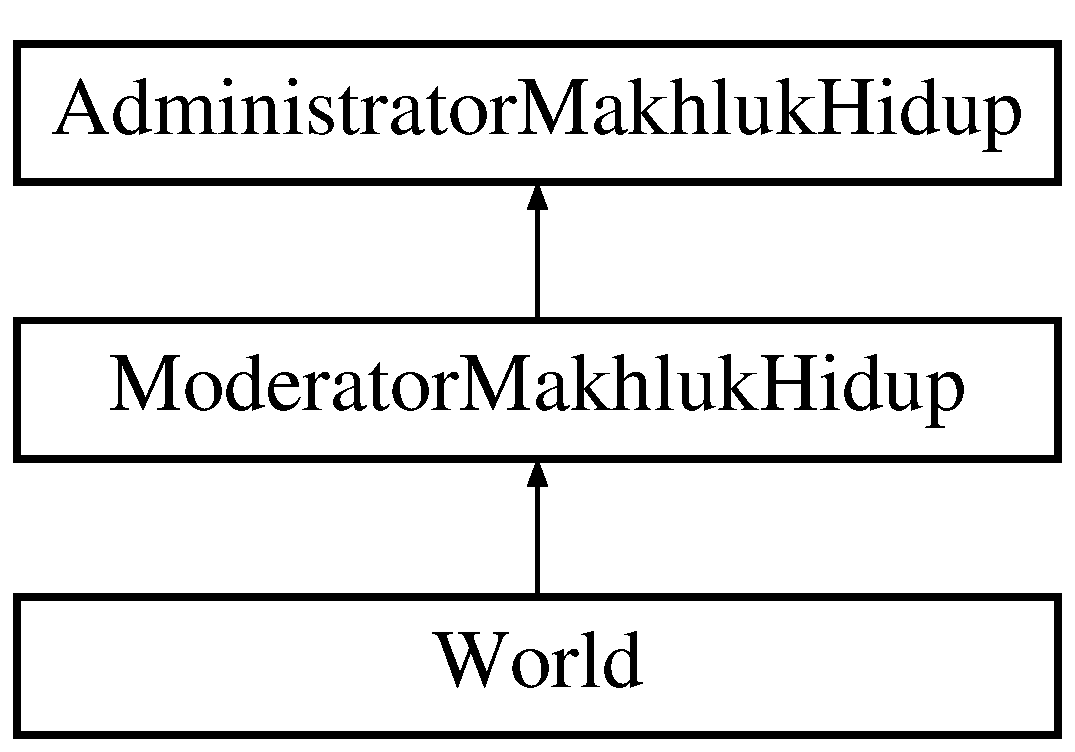
\includegraphics[height=3.000000cm]{class_moderator_makhluk_hidup}
\end{center}
\end{figure}
\subsection*{Public Member Functions}
\begin{DoxyCompactItemize}
\item 
void {\bfseries signal\+Position} ()\hypertarget{class_moderator_makhluk_hidup_ab230361c7f172ca30d8304cc5bf80ebf}{}\label{class_moderator_makhluk_hidup_ab230361c7f172ca30d8304cc5bf80ebf}

\end{DoxyCompactItemize}


The documentation for this class was generated from the following files\+:\begin{DoxyCompactItemize}
\item 
C\+:/\+Users/\+C\+X\+X\+X\+V/\+Documents/\+Git\+Hub/\+Makhluk/moderator\+Makhluk\+Hidup.\+h\item 
C\+:/\+Users/\+C\+X\+X\+X\+V/\+Documents/\+Git\+Hub/\+Makhluk/moderator\+Makhluk\+Hidup.\+cpp\end{DoxyCompactItemize}

\hypertarget{class_omnivora}{}\section{Omnivora Class Reference}
\label{class_omnivora}\index{Omnivora@{Omnivora}}
Inheritance diagram for Omnivora\+:\begin{figure}[H]
\begin{center}
\leavevmode
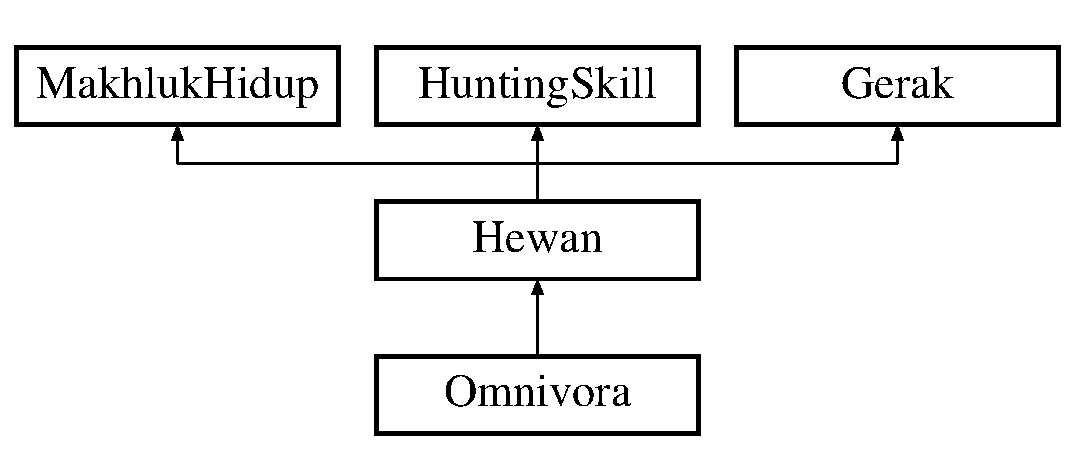
\includegraphics[height=3.000000cm]{class_omnivora}
\end{center}
\end{figure}
\subsection*{Public Member Functions}
\begin{DoxyCompactItemize}
\item 
virtual void {\bfseries memuda} ()=0\hypertarget{class_omnivora_a811aacb0d623b6c0ecc4a2fe80179a8b}{}\label{class_omnivora_a811aacb0d623b6c0ecc4a2fe80179a8b}

\end{DoxyCompactItemize}


The documentation for this class was generated from the following file\+:\begin{DoxyCompactItemize}
\item 
C\+:/\+Users/\+C\+X\+X\+X\+V/\+Documents/\+Git\+Hub/\+Makhluk/Omnivora.\+h\end{DoxyCompactItemize}

\hypertarget{class_point}{}\section{Point Class Reference}
\label{class_point}\index{Point@{Point}}
\subsection*{Public Member Functions}
\begin{DoxyCompactItemize}
\item 
{\bfseries Point} (int \+\_\+x=0, int \+\_\+y=0)\hypertarget{class_point_adbd2637ceed85e28315d96c8208154a5}{}\label{class_point_adbd2637ceed85e28315d96c8208154a5}

\item 
\hyperlink{class_point}{Point} \& {\bfseries operator=} (const \hyperlink{class_point}{Point} \&)\hypertarget{class_point_a55eeab949e62268da63176d48570eb54}{}\label{class_point_a55eeab949e62268da63176d48570eb54}

\item 
bool {\bfseries operator==} (const \hyperlink{class_point}{Point} \&)\hypertarget{class_point_a9201e61e7884cb0f861f09639cb1c121}{}\label{class_point_a9201e61e7884cb0f861f09639cb1c121}

\item 
void {\bfseries geser} (int dx, int dy)\hypertarget{class_point_ad2432ee1f003f107b898243a1285a14b}{}\label{class_point_ad2432ee1f003f107b898243a1285a14b}

\item 
int {\bfseries get\+Absis} ()\hypertarget{class_point_ae33b5d39a797830928a7d38376b23d21}{}\label{class_point_ae33b5d39a797830928a7d38376b23d21}

\item 
int {\bfseries get\+Ordinat} ()\hypertarget{class_point_a23af70007db8db0ac9f74d1eafecdadc}{}\label{class_point_a23af70007db8db0ac9f74d1eafecdadc}

\item 
void {\bfseries set\+Absis} (int \+\_\+x)\hypertarget{class_point_add1782a8109328ad174a8bc829621011}{}\label{class_point_add1782a8109328ad174a8bc829621011}

\item 
void {\bfseries set\+Ordinat} (int \+\_\+y)\hypertarget{class_point_adcb07a7e64713bc497e5174b5bec6a10}{}\label{class_point_adcb07a7e64713bc497e5174b5bec6a10}

\end{DoxyCompactItemize}


The documentation for this class was generated from the following files\+:\begin{DoxyCompactItemize}
\item 
Point.\+h\item 
Point.\+cpp\end{DoxyCompactItemize}

\hypertarget{class_polisi}{}\section{Polisi Class Reference}
\label{class_polisi}\index{Polisi@{Polisi}}


{\ttfamily \#include $<$Polisi.\+h$>$}

Inheritance diagram for Polisi\+:\begin{figure}[H]
\begin{center}
\leavevmode
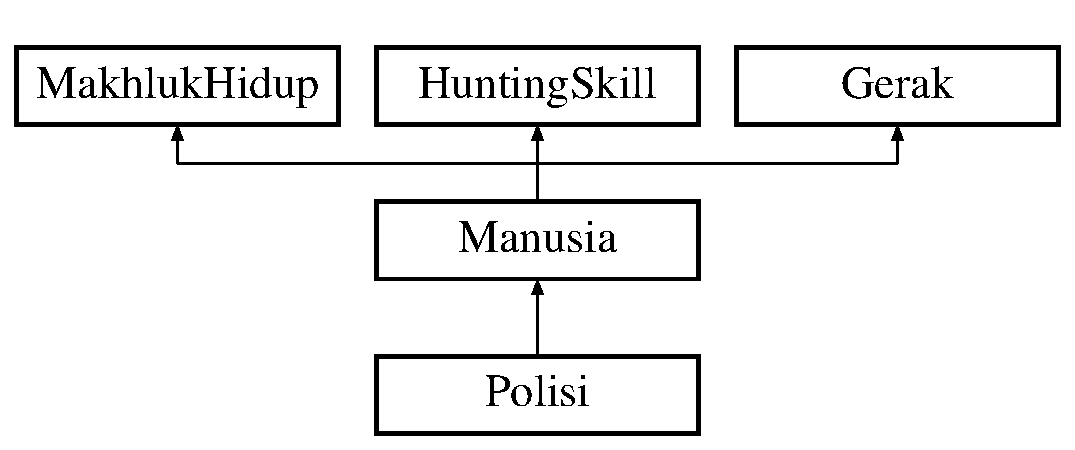
\includegraphics[height=3.000000cm]{class_polisi}
\end{center}
\end{figure}
\subsection*{Public Member Functions}
\begin{DoxyCompactItemize}
\item 
\hyperlink{class_polisi_ae7089485dba08278fd1df6d656e6da5b}{Polisi} (\hyperlink{class_point}{Point} P)
\item 
\hyperlink{class_polisi_aff98fa5fae4b27dfe99689359a8b8735}{Polisi} (const \hyperlink{class_polisi}{Polisi} \&)
\item 
\hyperlink{class_polisi}{Polisi} \& \hyperlink{class_polisi_a99d9244b99d637a32adef49f569d53d2}{operator=} (const \hyperlink{class_polisi}{Polisi} \&)
\item 
void \hyperlink{class_polisi_ad8c80d834481138e1fe1e8b62fad77bd}{Reaction} (\hyperlink{class_makhluk_hidup}{Makhluk\+Hidup} \&)
\end{DoxyCompactItemize}


\subsection{Detailed Description}
Class for constructing a human called \hyperlink{class_polisi}{Polisi} /$\ast$ 

\subsection{Constructor \& Destructor Documentation}
\index{Polisi@{Polisi}!Polisi@{Polisi}}
\index{Polisi@{Polisi}!Polisi@{Polisi}}
\subsubsection[{\texorpdfstring{Polisi(\+Point P)}{Polisi(Point P)}}]{\setlength{\rightskip}{0pt plus 5cm}Polisi\+::\+Polisi (
\begin{DoxyParamCaption}
\item[{{\bf Point}}]{P}
\end{DoxyParamCaption}
)}\hypertarget{class_polisi_ae7089485dba08278fd1df6d656e6da5b}{}\label{class_polisi_ae7089485dba08278fd1df6d656e6da5b}
ctor that take one argument to set the position of the \hyperlink{class_polisi}{Polisi} 
\begin{DoxyParams}{Parameters}
{\em A} & \hyperlink{class_point}{Point} \\
\hline
\end{DoxyParams}
\index{Polisi@{Polisi}!Polisi@{Polisi}}
\index{Polisi@{Polisi}!Polisi@{Polisi}}
\subsubsection[{\texorpdfstring{Polisi(const Polisi \&)}{Polisi(const Polisi &)}}]{\setlength{\rightskip}{0pt plus 5cm}Polisi\+::\+Polisi (
\begin{DoxyParamCaption}
\item[{const {\bf Polisi} \&}]{P}
\end{DoxyParamCaption}
)}\hypertarget{class_polisi_aff98fa5fae4b27dfe99689359a8b8735}{}\label{class_polisi_aff98fa5fae4b27dfe99689359a8b8735}
A copy constructor 

\subsection{Member Function Documentation}
\index{Polisi@{Polisi}!operator=@{operator=}}
\index{operator=@{operator=}!Polisi@{Polisi}}
\subsubsection[{\texorpdfstring{operator=(const Polisi \&)}{operator=(const Polisi &)}}]{\setlength{\rightskip}{0pt plus 5cm}{\bf Polisi} \& Polisi\+::operator= (
\begin{DoxyParamCaption}
\item[{const {\bf Polisi} \&}]{P}
\end{DoxyParamCaption}
)}\hypertarget{class_polisi_a99d9244b99d637a32adef49f569d53d2}{}\label{class_polisi_a99d9244b99d637a32adef49f569d53d2}
An operator= \index{Polisi@{Polisi}!Reaction@{Reaction}}
\index{Reaction@{Reaction}!Polisi@{Polisi}}
\subsubsection[{\texorpdfstring{Reaction(\+Makhluk\+Hidup \&)}{Reaction(MakhlukHidup &)}}]{\setlength{\rightskip}{0pt plus 5cm}void Polisi\+::\+Reaction (
\begin{DoxyParamCaption}
\item[{{\bf Makhluk\+Hidup} \&}]{M}
\end{DoxyParamCaption}
)\hspace{0.3cm}{\ttfamily [virtual]}}\hypertarget{class_polisi_ad8c80d834481138e1fe1e8b62fad77bd}{}\label{class_polisi_ad8c80d834481138e1fe1e8b62fad77bd}
A procedure that make the \hyperlink{class_polisi}{Polisi} react to the other \hyperlink{class_makhluk_hidup}{Makhluk\+Hidup} 
\begin{DoxyParams}{Parameters}
{\em \hyperlink{class_makhluk_hidup}{Makhluk\+Hidup}} & \\
\hline
\end{DoxyParams}


Implements \hyperlink{class_makhluk_hidup_a7aafd6122203f48a43b384a9d8175396}{Makhluk\+Hidup}.



The documentation for this class was generated from the following files\+:\begin{DoxyCompactItemize}
\item 
Polisi.\+h\item 
Polisi.\+cpp\end{DoxyCompactItemize}

\hypertarget{class_world}{}\section{World Class Reference}
\label{class_world}\index{World@{World}}
Inheritance diagram for World\+:\begin{figure}[H]
\begin{center}
\leavevmode
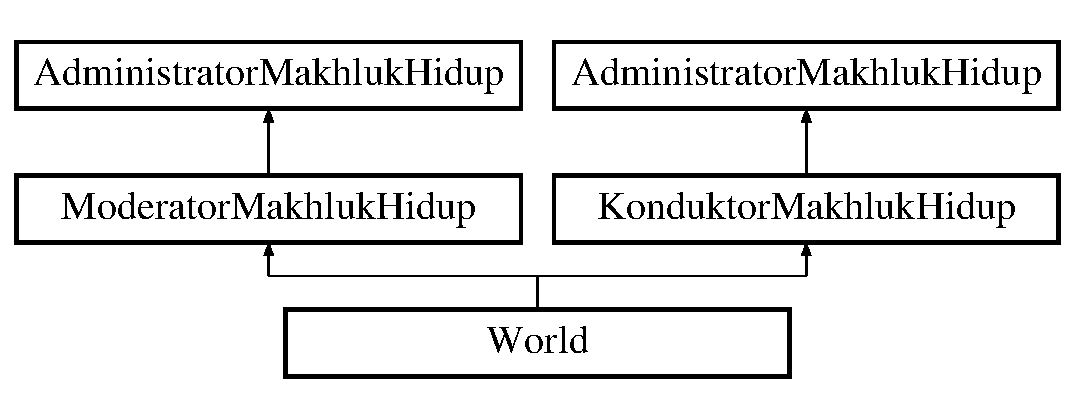
\includegraphics[height=3.000000cm]{class_world}
\end{center}
\end{figure}
\subsection*{Public Member Functions}
\begin{DoxyCompactItemize}
\item 
void {\bfseries init\+Display} ()\hypertarget{class_world_a3ccab52e143cc85200d3d4a5384c4559}{}\label{class_world_a3ccab52e143cc85200d3d4a5384c4559}

\item 
void {\bfseries update\+Display} ()\hypertarget{class_world_a0656cc8aa64881db8880d6a1af0d5aea}{}\label{class_world_a0656cc8aa64881db8880d6a1af0d5aea}

\item 
bool {\bfseries game\+Over} ()\hypertarget{class_world_a49e876669efe76ffb57bd0bd70370151}{}\label{class_world_a49e876669efe76ffb57bd0bd70370151}

\end{DoxyCompactItemize}


The documentation for this class was generated from the following files\+:\begin{DoxyCompactItemize}
\item 
C\+:/\+Users/\+C\+X\+X\+X\+V/\+Documents/\+Git\+Hub/\+Makhluk/world.\+h\item 
C\+:/\+Users/\+C\+X\+X\+X\+V/\+Documents/\+Git\+Hub/\+Makhluk/world.\+cpp\end{DoxyCompactItemize}

%--- End generated contents ---

% Index
\backmatter
\newpage
\phantomsection
\clearemptydoublepage
\addcontentsline{toc}{chapter}{Index}
\printindex

\end{document}
